%% 
%% Copyright 2007-2025 Elsevier Ltd
%% 
%% This file is part of the 'Elsarticle Bundle'.
%% ---------------------------------------------
%% 
%% It may be distributed under the conditions of the LaTeX Project Public
%% License, either version 1.3 of this license or (at your option) any
%% later version.  The latest version of this license is in
%%    http://www.latex-project.org/lppl.txt
%% and version 1.3 or later is part of all distributions of LaTeX
%% version 1999/12/01 or later.
%% 
%% The list of all files belonging to the 'Elsarticle Bundle' is
%% given in the file `manifest.txt'.
%% 
%% Template article for Elsevier's document class `elsarticle'
%% with harvard style bibliographic references

% \documentclass[preprint,12pt]{elsarticle}

%% Use the option review to obtain double line spacing
\documentclass[preprint,review,12pt]{elsarticle}

%% Use the options 1p,twocolumn; 3p; 3p,twocolumn; 5p; or 5p,twocolumn
%% for a journal layout:
%% \documentclass[final,1p,times]{elsarticle}
% \documentclass[final,1p,times,twocolumn]{elsarticle}
%% \documentclass[final,3p,times]{elsarticle}
%%\documentclass[final,4p,times,twocolumn]{elsarticle}
%% \documentclass[final,5p,times]{elsarticle}
% \documentclass[final,5p,times,twocolumn]{elsarticle}

%% For including figures, graphicx.sty has been loaded in
%% elsarticle.cls. If you prefer to use the old commands
%% please give \usepackage{epsfig}

%% The amssymb package provides various useful mathematical symbols

\usepackage{multirow}

\usepackage{tikz}
\usetikzlibrary{shapes.geometric, arrows.meta, positioning}

\tikzstyle{startstop} = [rectangle, rounded corners, minimum width=3cm, minimum height=1cm,text centered, draw=black, fill=blue!20]
\tikzstyle{process} = [rectangle, minimum width=3.5cm, minimum height=1cm, text centered, draw=black, fill=orange!30]
\tikzstyle{decision} = [diamond, aspect=2, minimum width=3cm, minimum height=1cm, text centered, draw=black, fill=green!30]
\tikzstyle{arrow} = [thick,->,>=stealth]


\usepackage{amssymb}

%% The amsmath package provides various useful equation environments.
\usepackage{amsmath}
\usepackage{cleveref}
\usepackage{stfloats}

\usepackage{float}
\usepackage{placeins}
%% The amsthm package provides extended theorem environments
%% \usepackage{amsthm}

%% The lineno packages adds line numbers. Start line numbering with
%% \begin{linenumbers}, end it with \end{linenumbers}. Or switch it on
%% for the whole article with \linenumbers.
%% \usepackage{lineno}

\journal{Nuclear Physics B}

\begin{document}

\begin{frontmatter}

%% Title, authors and addresses

%% use the tnoteref command within \title for footnotes;
%% use the tnotetext command for theassociated footnote;
%% use the fnref command within \author or \affiliation for footnotes;
%% use the fntext command for theassociated footnote;
%% use the corref command within \author for corresponding author footnotes;
%% use the cortext command for theassociated footnote;
%% use the ead command for the email address,
%% and the form \ead[url] for the home page:
% \title{Title\tnoteref{label1}}
%% \tnotetext[label1]{}
%% \author{Name\corref{cor1}\fnref{label2}}
%% \ead{email address}
%% \ead[url]{home page}
%% \fntext[label2]{}
%% \cortext[cor1]{}
%% \affiliation{organization={},
%%             addressline={},
%%             city={},
%%             postcode={},
%%             state={},
%%             country={}}
%% \fntext[label3]{}

\title{Fission Matrix Method for Criticality Search in Heat-Pipe Micro Reactors} %% Article title

%% use optional labels to link authors explicitly to addresses:
\author[label1]{Christian Vita}
\author[label1]{Nicolo' Abrate} %% Author name
\author[label1]{Sandra Dulla} %% Author name
\author[label5,label6]{Valerio Mascolino} %% Author name
\author[label3]{William Walters} %% Author name
\author[label2]{Nicolas Stauff}
\author[label4]{Fausto Franceschini}

\affiliation[label1]{organization={NEMO group, Energy Department, Politecnico di Torino},
            addressline={Corso Duca degli Abruzzi 24},
            city={Turin},
            postcode={10129},
            state={Italy},
            country={}}

\affiliation[label2]{organization={Argonne National Laboratory },
            addressline={},
            city={Lemont},
            postcode={},
            state={IL},
            country={USA}}

\affiliation[label3]{organization={Westinghouse Electric Company},
            addressline={},
            city={Cranberry},
            postcode={},
            state={PA},
            country={USA}}
            
\affiliation[label4]{organization={Westinghouse Mangiarotti},
            addressline={v. Timavo 59},
            city={Monfalcone},
            postcode={34074},
            state={Italy},
            country={}}

\affiliation[label5]{organization={Nuclear Science and Engineering},
            addressline={Colorado School of Mines},
            city={Golden},
            postcode={80401},
            state={CO},
            country={USA}}

\affiliation[label6]{organization={Department of Mechanical Engineering},
            addressline={Colorado School of Mines},
            city={Golden},
            postcode={80401},
            state={CO},
            country={USA}}


%% Abstract
\begin{abstract}
%% Text of abstract
The Fission Matrix (FM) method is applied to conduct the neutronics analysis of the VTB Heat-Pipe Micro Reactor (HPMR). The aim of this model is to support the design of heat-pipe-based microreactors, which are gaining significant interest from the industry.

A database of FMs is generated at various uniform temperatures and Control Drum (CD) rotation angles using Monte Carlo simulations with Serpent2. This database is then used to interpolate FMs at intermediate conditions not explicitly included in the dataset. By solving the eigenvalue problem of the interpolated FM, the corresponding effective multiplication factor ($k_{eff}$) and fission source distribution ($F(\vec{r})$) are obtained.

The accuracy of the interpolated results is assessed by comparison with reference Serpent2 simulations. The analysis is conducted under various temperature distributions and CD positions. The study also highlights the negative impact on accuracy caused by large temperature differences between the core and the reflector. To address this, a correction ratio is defined, which requires only a relatively small number of additional FMs to be added to the database.

Leveraging the computational efficiency and high accuracy of the FM approach, a custom criticality search algorithm is developed. The interpolated FMs are solved iteratively, updating the CD positions and the resulting temperature distribution until criticality is achieved ($k_{eff} = 1$).

\end{abstract}


%% Keywords
\begin{keyword}

Fission matrix \sep criticality search \sep heat-pipe micro reactor \sep VTB HPMR \sep correction ratio . 

\end{keyword}



\end{frontmatter}

%% Add \usepackage{lineno} before \begin{document} and uncomment 
%% following line to enable line numbers
%% \linenumbers

%% main text
%%

%% Use \section commands to start a section
\section{Introduction} \label{section:Introduction}
%% Labels are used to cross-reference an item using \ref command.

Monte Carlo softwares are regarded as one of the most precise tools for neutronics calculations due to their capacity to employ continuous angle and energy variables and accurately model geometries. Nevertheless, these simulations incur substantial computational expense because they rely on stochastic simulations of individual particles, particularly when striving for acceptable uncertainty levels of the results. This computational burden turns Monte Carlo methods less practical for applications that requires high number of calculations, such as transient simulations, criticality search algorithm or different design purposes.

To overcome this, an alternative approach have been proposed, based on the fission matrix concept which requires the model to be subdivided into $N$ cells, used to tally the average number of neutrons generated in the i-th cell due to the fission reaction of one neutron born in the j-th cell. These information are collected in a $N$x$N$ matrix ($\textbf{A}$), called fission matrix.  In multiplying systems, the principal eigenvector $F_0(\vec{r})$ of the fission matrix $\textbf{A}$ represents the fission source distribution, while its principal eigenvalue corresponds to the multiplication factor $k_{eff}$.
The FM method has been used a wide and different number of studies, such as spent-fuel pools, whole-core power reactor calculations, transient simulations of novel reactor designs, nuclear thermal propulsion reactors, and research reactors \cite{Walters2018}, \cite{Wang2018}, \cite{Mascolino2022}.

The Fission matrix method have been suggested also as a means to eliminate inactive cycles in Monte Carlo calculations and to achieve unbiased solutions in problems characterized by high dominance ratios; this capability, however, is not object of analysis of this study.

The goal of this work is to use the FM method to the VTB HPMR design- described in the next section. The purpose is to demonstrate that the method can be applied also for this type of advance reactor design, especially when 3D temperature distribution and control drums positions are considered. Once the accuracy of the method is analyzed, it is leveraged to define a fast and accurate criticality search algorithm. 


\subsection{VTB HPMR Model} \label{section:VTB HPMR model}
The model is based on the Micro-Reactor design under analysis by the NEAMS Micro-Reactor Application Drivers area (\cite{Stauff2024}). As a modeling exercise, the micro-reactor concept was designed at ANL to gather some of the most pressing modeling challenges faced by the micro-reactor industry, which are:  The use of heat pipe technologies to remove the nuclear heat, the use of TRi-structural ISOtropic (TRISO) fuel to enable operations at very high temperatures and the use of rotating control rod drums in the radial reflectors. 

The reactor core is designed for a rated thermal power of 2 MW, and its configuration is illustrated in the figure below. The fuel adopted is a conventional TRISO type, containing 19.95 at\% Low-Enriched Uranium (LEU) in UCO form, embedded within a hexagonal graphite matrix at a packing fraction of 40\%. The active core length is 160 cm, bounded axially by 20 cm beryllium metal reflectors at both the top and bottom. The core consists of 30 fuel assemblies, arranged within a single ring of beryllium radial reflector and 12 rotating control drums. To reduce computational effort, only one-sixth of the core geometry is modeled.

To optimize neutron moderation, yttrium-hydride (YH$_2$) pins are incorporated alongside the graphite structural components. Due to its superior neutron slowing-down properties, YH$_2$ enables a more compact core design. The YH$_2$ pins are encased in a stainless steel cladding, with a helium gap between the hydride and the cladding, as well as an additional gap between the cladding and the surrounding graphite monolith.

The heat removal system utilizes heat pipes composed of a stainless steel envelope and potassium as the working fluid. A helium gap thermally isolates each heat pipe from the graphite monolith. Radially, each heat pipe is divided into three functional zones: a vapor core, a liquid-plus-wick region, and the outer envelope.

The reactor control system features 12 control drums embedded within the radial reflector, providing full control capability, including cold shutdown, under all operational conditions. For additional redundancy, a dedicated shutdown rod is positioned at the center of the core.


\begin{figure}[t]
\centering
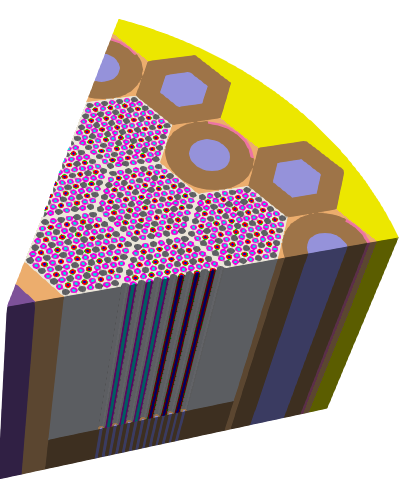
\includegraphics[scale=0.65]{images/VTB_fullcore_3D_slice_sextant.png}  % Modifica scale o usa width se serve
\caption{VTB core, considering only one sextant of the geometry.}
\label{fig1}
\end{figure}



\section{Methodology} \label{section:Methodology}

\subsection{Fission Matrix Definition} \label{subsection:Fission matrix definition}
The fission matrix is generated through a Monte Carlo code, which in this study is Serpent2 \cite{LEPPANEN2025}.
To define the fission matrix, the user is required to discretize into $N$ spatial cells, each used to tally the average number of neutrons produced in the $i$-th cell as a result of a fission event initiated by a neutron born in the $j$-th cell. This set of interactions is stored in an $N \times N$ matrix $\textbf{A}$, known as the fission matrix. In multiplying systems, the dominant eigenvector $F_0(\vec{r})$ (from hereafter it will be denoted just as $F$) of $\textbf{A}$ represents the steady-state fission source distribution, while its associated eigenvalue corresponds to the effective multiplication factor, $k_{eff}$ \cite{Carney2014}. The eigenproblem can then be formulated as follows:

\begin{equation}
F_i = \frac{1}{k_{eff}}\sum_j^N a_{ij}F_j .
\end{equation}

Usually, a pin-wise Cartesian mesh is adopted to tally the FM; however, in this study, such a level of detail of the fission matrix and consequently of the fission source is not needed: an assembly-wise detail is sufficient for this study.
Moreover, a Cartesian mesh easily allows overlapping the actual position of the fissile elements with the mesh cells (whether pin-level or assembly-level) with square-lattice system. However, the HPMR adopts a hexagonal lattice. In Serpent2, the fission matrix can be tallied only over Cartesian meshes. To overcome this limitation, the Serpent2 feature to generate a material-based fission matrix is used. Thanks to this capability, the tallying is done material-wise: the number of neutrons emitted by a fission reaction in the $i$-th fissile material because of a neutron born in the $j$-th fissile material. Relying on this feature, it is possible to work around the limitation of the square mesh to tally the fission matrix, by combining the fission matrix material-based option with the \texttt{div} card to differentiate the fuel material for each core assembly and for an arbitrary number of axial cuts. In total, the core has 30 fuel assemblies and 3 axial regions are defined in this study; hence, a total of 90 cells are used and the fission matrix has 90×90 items.



\subsection{Database Definition} \label{subsection:Database definition}
The FM method, need a certain upfront computational burden to generate the Fission Matrix DataBase (FMDB). The amount of calculation depends on the number or parameters that are considered to be relevant to be accounted for in the analysis.
In this specific case, two key parameters are considered: the fuel temperature and the position of the control drums.

It is important to specify that each temperature value in the database represents a uniform temperature applied to the entire reactor system. That is, no spatial temperature gradients are considered; the fuel, moderator, and structural components are all assumed to be at the same temperature for each database entry. Similarly, the control drum (CD) position is represented by a single rotation angle, which is equally applied to all control drums. This means that in each configuration, all CDs are rotated by the same angle, preserving a symmetric control strategy.

One of the challenges of defining the FMDB is that it is not known apriori the minimum amount of data needed to have a sufficiently accurate results. This problem is accounted in the results section.   

\subsection{FM Interpolation}
Since two variables are considered to vary in the FMDB, a bivariate interpolation scheme is required. As a preliminary approach, a simple bivariate linear interpolation is adopted. However, it is important to highlight that more advanced interpolation schemes could potentially yield better results. In other words, they could allow for a more efficient use of the FMDB by reducing the number of data points required to achieve the same level of accuracy as with linear interpolation. Nevertheless, implementing such advanced schemes requires a dedicated study, which is beyond the scope of this work.

The bivariate linear interpolation used to obtain the element $\tilde{a}_{ij}$ of the interpolated fission matrix $\tilde{\mathbf{A}}$ is defined as:

\begin{align}
\tilde{a}_{ij}(\tilde{T}_{f,i}, \tilde{\theta}) =&\; a_{ij}^{(d_T, d_{\theta})}
\left( \frac{T_{f,i}^{(d_T+1)} - \tilde{T}_{f,i}}{T_{f,i}^{(d_T+1)} - T_{f,i}^{(d_T)}} \right)
\left( \frac{\theta^{(d_{\theta}+1)} - \tilde{\theta}}{\theta^{(d_{\theta}+1)} - \theta^{(d_{\theta})}} \right) \notag \\
&+ a_{ij}^{(d_T+1, d_{\theta})}
\left( \frac{\tilde{T}_{f,i} - T_{f,i}^{(d_T)}}{T_{f,i}^{(d_T+1)} - T_{f,i}^{(d_T)}} \right)
\left( \frac{\theta^{(d_{\theta}+1)} - \tilde{\theta}}{\theta^{(d_{\theta}+1)} - \theta^{(d_{\theta})}} \right) \notag \\
&+ a_{ij}^{(d_T, d_{\theta}+1)}
\left( \frac{T_{f,i}^{(d_T+1)} - \tilde{T}_{f,i}}{T_{f,i}^{(d_T+1)} - T_{f,i}^{(d_T)}} \right)
\left( \frac{\tilde{\theta} - \theta^{(d_{\theta})}}{\theta^{(d_{\theta}+1)} - \theta^{(d_{\theta})}} \right) \notag \\
&+ a_{ij}^{(d_T+1, d_{\theta}+1)}
\left( \frac{\tilde{T}_{f,i} - T_{f,i}^{(d_T)}}{T_{f,i}^{(d_T+1)} - T_{f,i}^{(d_T)}} \right)
\left( \frac{\tilde{\theta} - \theta^{(d_{\theta})}}{\theta^{(d_{\theta}+1)} - \theta^{(d_{\theta})}} \right)
\end{align}

where:
\begin{itemize}
  \item $\tilde{a}_{ij}$: interpolated element of the fission matrix $\tilde{\mathbf{A}}$,
  \item $d_T$, $d_{\theta}$: indices such that $\tilde{T}_f \in [T_f^{(d_T)}, T_f^{(d_T+1)}]$ and $\tilde{\theta} \in [\theta^{(d_{\theta})}, \theta^{(d_{\theta}+1)}]$  ,
  \item $a_{ij}^{(d_T, d_{\theta})}$: known value of the element at grid point $(T_f^{(d_T)}, \theta^{(d_{\theta})})$,
  \item $\tilde{T}_{f,i}$: target fuel temperature at cell "$i$" for interpolation,
  \item $\tilde{\theta}$: target CDs angle for interpolation,
  \item $T_f^{(d_T)}$, $T_f^{(d_T+1)}$: adjacent temperature grid points in the FMDB,
  \item $\theta^{(d_{\theta})}$, $\theta^{(d_{\theta}+1)}$: adjacent angle grid points.
\end{itemize}


\subsection{Core Reflector Treatment: Definition of the Reflector Correction Ratio}
In nuclear reactors, neutron reflectors are employed to reduce neutron leakage by scattering escaping neutrons back into the core, thereby enhancing the overall neutron economy. This allows for more efficient fuel utilization and contributes to maintaining criticality with less fissile material. In the context of Heat Pipe Micro Reactors (HPMRs), reflectors play an even more critical role due to the compactness of the core and the limited amount of fissile material, strongly affecting the neutron flux shape.

Due to the definition of the fission matrix, temperature can only be imposed on the fuel assemblies during interpolation. Moreover, the database used in this study assumes a uniform temperature distribution across the entire system. As a result, when analyzing more realistic cases that include a temperature gradient between the fuel and the reflector, the method may yield less accurate results. To address this limitation, a Reflector Correction Ratio (RCR) is defined, similarly to what has done in \cite{Rau2020} but focusing the definition and application of the correction on the temperature difference between core and reflector, which plays a crucial role, especially for in HPMRs. The idea is to directly multiply the already-generated $\tilde{\textbf{A}}$ with the matrix $\textbf{R}$, which contains the correction ratios of each element of the fission matrix, such that: 


\begin{equation}
\tilde{\textbf{A}}^{*} F^{*} = \textbf{R}\tilde{\textbf{A}} F^* = \frac{1}{k^*_{eff}} F^*.
\end{equation}


Where each items of $\textbf{R}$ can be defined as: 

\begin{equation}
r_{i,j}(T_{f,i}, T_{r,i}, \theta) = \frac{T_{f,i} - T_{r,i}}{T_{max,DB} - T_{min,DB}} \cdot \left( \frac{ \tilde{a_{i,j}}(T_{f,i}, \theta)}{a_{i,j}^{\Delta T}} - 1 \right) + 1
\label{eq:correction_ratio_1}
\end{equation}

Where: 

\begin{itemize}
    \item $T_{r,i}$: Temperature of the closest non-fissile cell to fissile cell '$i$'. 
    \item $ \theta $: Cosine of the CD rotation angle.     
    \item $T_{max,DB}$: Maximum temperature used in the uniform distribution used in the database.  
    \item $T_{min,DB}$: Minimum temperature used in the uniform distribution used in the database 
    \item $a_{i,j}^{\Delta T}$: Fission matrix with $T_{f}=1000$K and $T_{r}=300$K.   
\end{itemize}

Given this formulation, an additional simulation is required to obtain the latest variable and, thus to define the correction ratio. This additional case is a relatively limited additional computational effort considering the burden of generating the whole FMDB.  
However, heat pipe microreactors typically adopt a control mechanism based on control drums positioned outside the core, specifically within the reflector region. This design choice significantly influences the neutron flux distribution, particularly at the interface between the reflector and the outermost ring of fuel assemblies. When the control drums are rotated to introduce neutron-absorbing material into the reflector, a pronounced perturbation in the local neutron spectrum and leakage occurs in this boundary region. Thus, each time a CD is rotated, the correlation twen the reflector and the core, changes. In other terms, it would be as if, once the CDs assume a new position, the material, or better the material proportion at the interface of the system mutates, requiring a new  $a_{i,j}^{\Delta T}$ that describe this "new" system. 
This effect is not negligible, therefore, to more accurately capture the impact of control drum insertion the correction ratio introduced previously must be refined. 

To account for this additional complexity, \Cref{eq:correction_ratio_1} can be redefined as follows:    

\begin{equation}
r_{i,j}(T_{f,i}, T_{r,i}, \theta) = \frac{T_{f,i} - T_{r,i}}{T_{max,DB} - T_{min,DB}} \cdot \left( \frac{ \tilde{a_{i,j}}(T_{f,i}, \theta)}{a_{i,j}^{\Delta T}(\theta)} - 1 \right) + 1
\label{eq:correction_ratio_2}
\end{equation}

Accordingly, with respect to the original formulation in \Cref{eq:correction_ratio_1}, it is important to note that the coefficient $a_{i,j}^{\Delta T}$ now is a function of the parameter $\theta$. This dependency arises from the rotation-sensitive behavior of the system and the way thermal gradients interact with the geometric configuration of the core.

As a direct consequence, the denominator in the correction ratio equation must also be interpolated across different values of $\theta$. This modification introduces a significant refinement in the correction mechanism, as it adapts more effectively to the angular variation of the system’s response.

As a result, the total number of simulations required to construct the database and compute the correction ratio using the second formulation is:
\[
N_T N_{\theta} + N_{\theta}.
\]

Of course, \cref{eq:correction_ratio_2} is more expansive from the computational time point of view then the first formulation, however it is important to stress the fact that for control rods-based reactor designs, \cref{eq:correction_ratio_1} would be enough to improve results accuracy, since the peripheral region outside the core does not change during the operations of the reactor. The control rods are inserted inside the core to tune the reactivity of the system, which for sure causes strong neutron flux changes, and thus the FM's values, however these effects would be already accounted when different insertion steps are simulated to build the the FMDB.      


\subsection{Power and fuel temperature correlation}
To estimate the average fuel temperature corresponding to a given power level without performing a full thermal-hydraulic simulation for each case, a made-up correlation is defined. This approach is used to compute the temperature input for the fission matrix interpolation when the power of the system is varied. The correlation ensures, in a simple way, consistency between the power level and the fuel temperature used in the neutronics model, without requiring full thermal feedback calculations.

By assuming that fuel temperature scales linearly with power through a predefined relationship, and that the distribution itself is proportional to the fission source - $T_{f,i} \propto F_{i} $, the following correlation is defined:


\begin{align}
 &T_{f,i} =  \frac{P}{P_N} \xi_i  + T_{\min,DB}, 
 \\ &
\xi_i= \left[ \frac{F_i - \min(F)}{\max(F) - \min(F)} \cdot \Delta T_{\text{range}} + (T_{f,\min} - T_{\min,DB}) \right], 
\notag \\ &
 \text{with} \quad P \in [0,P_{\text{max}}].
\label{eq:correction_power_temperature}
\end{align}



Where: 

\begin{itemize}
    \item $P$: is the specific considered power. This can be seen as the free variable.
    \item $P_N$: is the nominal power of the reactor (2 MW). 
    \item $T_{f,i}$: temperature of the fissile cell '$i$'.
    \item $F$: fission source. 
    \item $\Delta T_{range} $: is the maximum temperature difference encountered inside the core at nominal power. This parameter has to be given as an input.     
    \item $T_{f,min}$: is the minimum temperature encountered inside the core at nominal power. This parameter has to be given as an input.  
    \item $T_{min,DB}$: minimum temperature used in the uniform distribution used in the database.   
\end{itemize}

This formulation is subject to a specific range of validity, as the power level must remain below an upper bound, denoted as \( P_{\text{max}} \). This constraint ensures that the resulting fuel temperature does not exceed the maximum temperature present in the database, which is limited to \( T_{\text{max,DB}} = 1000\,\text{K} \). Exceeding this threshold would need an extrapolation beyond the available data, which would reduce the reliability and physical consistency of the method. For this reason, the maximum allowable power \( P_{\text{max}} \) is explicitly defined as follows:



\begin{equation}
P_{\text{max}} = \frac{(T_{\text{max,DB}} - T_{\text{min,DB}})\cdot P_N}{\Delta T_{\text{range}} - (T_{\text{f,min}} - T_{\text{min,DB}})}
\label{eq:maximum_power_formulation}
\end{equation}

Thus, the maximum allowable input power depends on two parameters: $\Delta T_{\text{range}}$ and $T_{\text{f,min}}$. In \Cref{fig:parametric_limits_Pmax}, the parametric variation of the system’s upper power limit is shown. Once the parameters are chosen, all the points above the resulting curves, would make the temperature distribution exceeding the maximum temperature considered in the database (1000 K). Conversely, all points below the curve ensure that the temperature in every cell remains within the valid range of the database.

\begin{figure}[h!]
\centering
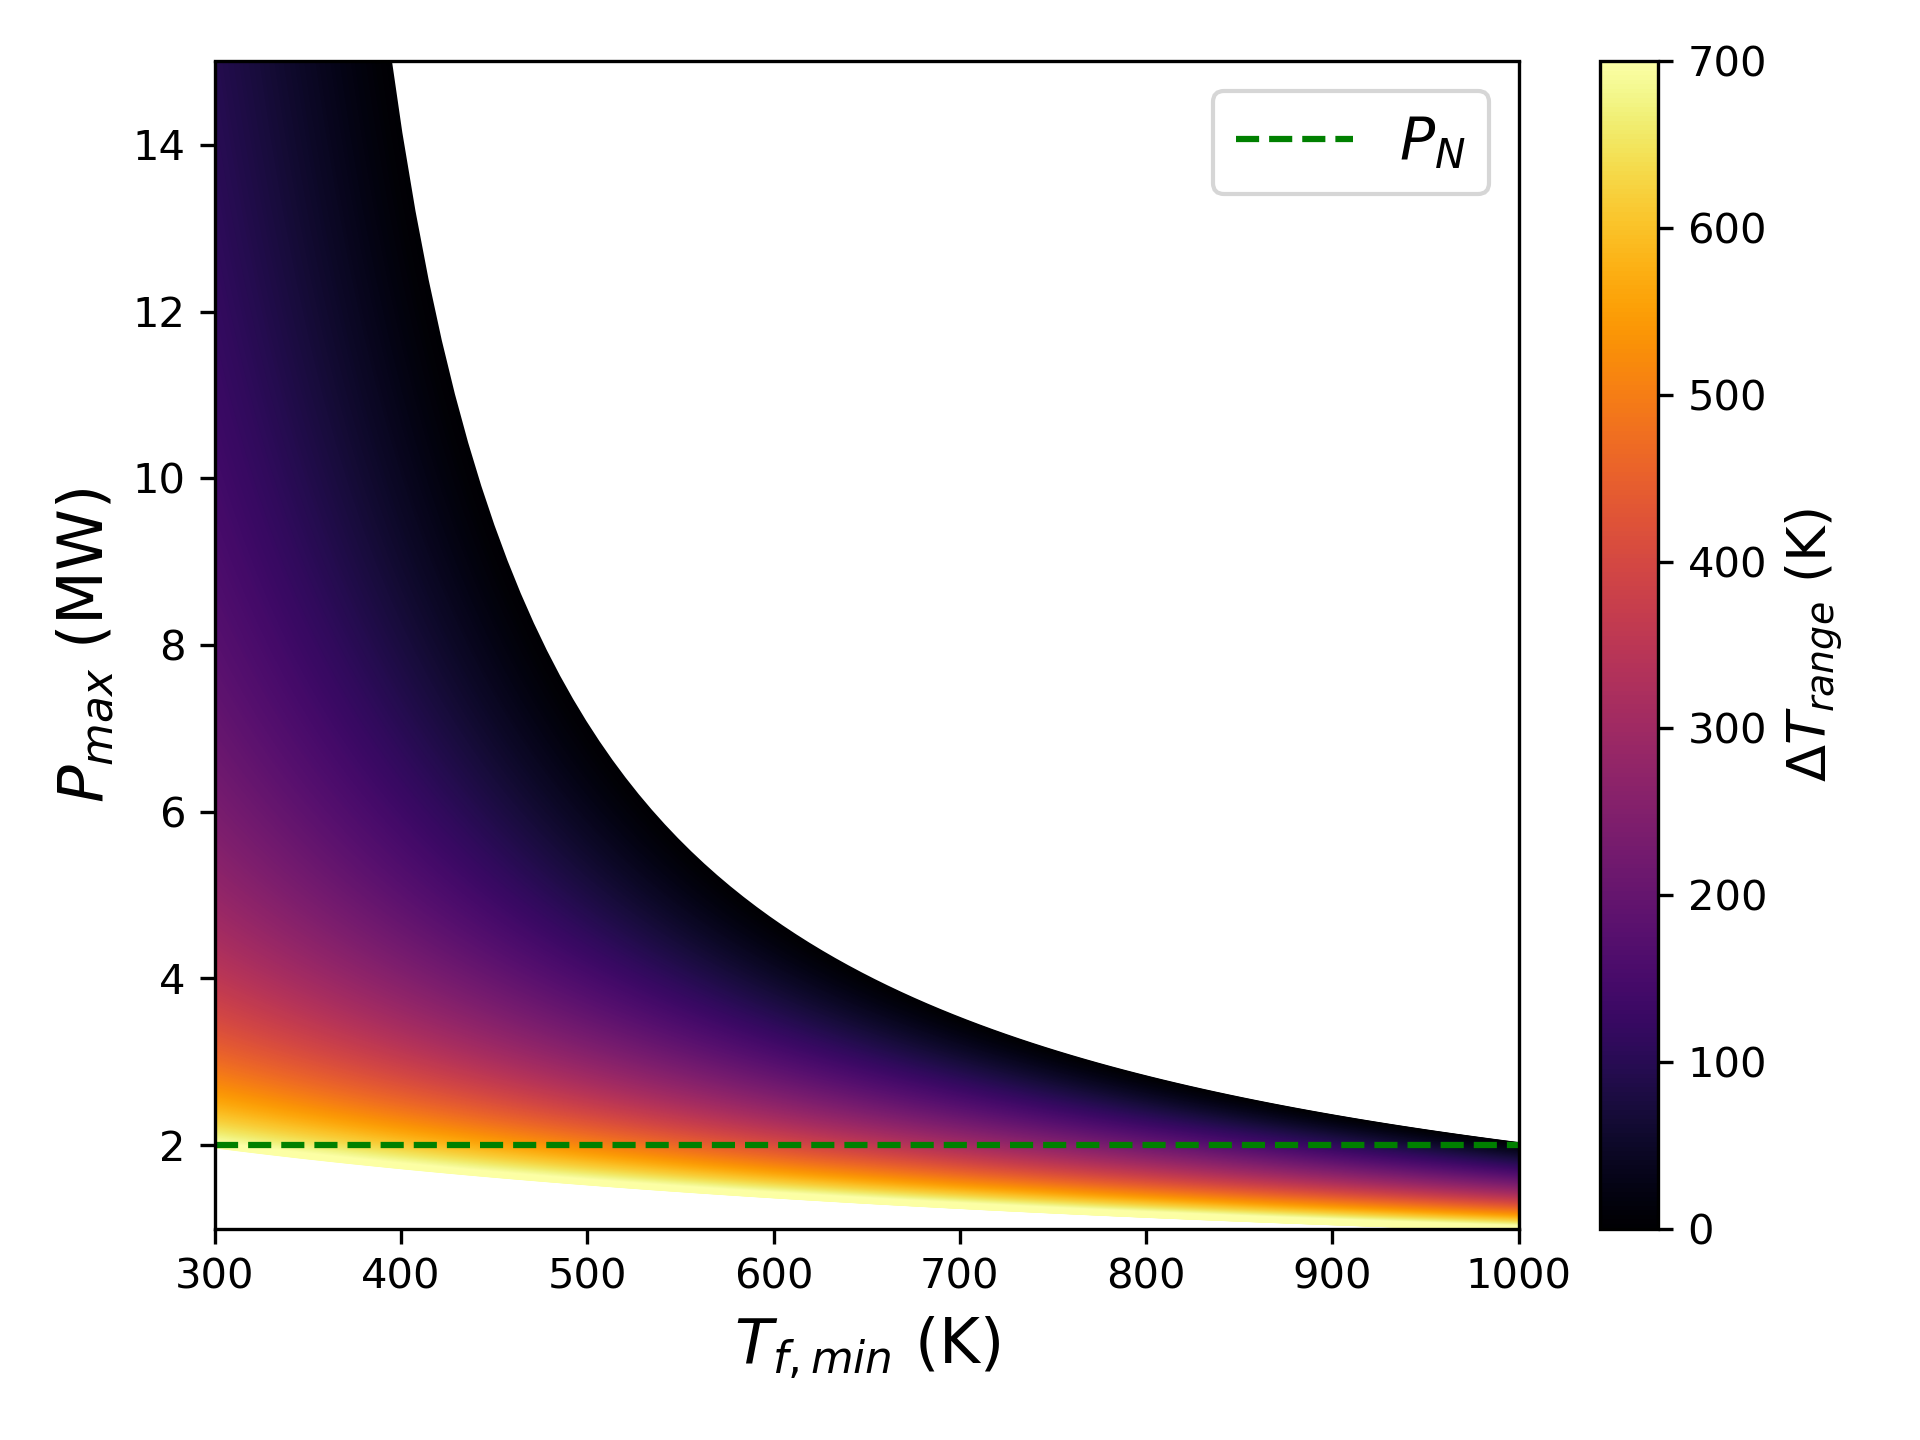
\includegraphics[scale=0.5]{images/parametric_limits_Pmax.png}  % Modifica scale o usa width se serve
\caption{Parametric $P_{\text{max}}$ domain visualization.}
\label{fig:parametric_limits_Pmax}
\end{figure}


\subsection{Criticality search algorithm}
\label{subsec:criticality_search_method}
Thanks to the correlation previously defined between power and fuel temperature, it is now possible to automate both the computation of the temperature distribution within the fuel and the criticality search involving the control drum positioning.

The criticality search algorithm aims to determine a configuration of the system in which the reactor reaches a critical state (i.e., $k_{eff} = 1$), while accounting for the thermal feedback on the neutron flux and the control drum (CD) positioning. The procedure includes two nested convergence loops: one for the temperature distribution and one for criticality itself. The algorithm steps, corresponding to the flowchart in \Cref{fig:crit_search_unified_loop}, are described below:

\begin{enumerate}
    \item \textbf{Initialization:} \\
    The algorithm begins by setting the control drum angle $\theta_{CD} = 0$, an initial guess for the power distribution $F_{\text{guess}}$, the minimum fuel temperature $T_{f,min}$, the maximum temperature difference observed inside the system, $\Delta T_{\text{range}}$, and the total power $P$.

    \item \textbf{Initial Temperature Calculation:} \\
    Based on the initial guess, the corresponding fuel temperature distribution $T_f$ is computed.

    \item \textbf{Power Distribution Calculation:} \\
    With the current temperature field, a new power distribution $F$ is computed using the neutronic solver or interpolation from a database (e.g., via a fission matrix).

    \item \textbf{Updated Temperature Calculation:} \\
    A new temperature profile is calculated using the updated power distribution $F$, considering thermal feedback.

    \item \textbf{Temperature Convergence Check:} \\
    The algorithm checks whether the new temperature profile differs from the previous one by less than a defined threshold $\epsilon$. In this study $\epsilon$ is set to 0.5\%. If the convergence is not satisfied:
    \begin{itemize}
        \item The temperature profile is updated.
        \item The algorithm returns to step 3 and continues iterating.
    \end{itemize}
    If convergence is achieved, the algorithm proceeds to the next step.

    \item \textbf{Criticality Convergence Check:} \\
    The previous $k_{eff}^{old}$ is updated with the current $k_{eff}^{new}$. The convergence condition $|k_{eff}^{new} - 1| < \delta$ is then checked:
    \begin{itemize}
        \item If not satisfied, the CD angle is adjusted and the algorithm returns to step 3.
        \item If satisfied, criticality is achieved, and the algorithm proceeds to the final step.
    \end{itemize}
    In this study $\delta$ is set to 1 pcm. 

    \item \textbf{Finalization:} \\
    Once both the temperature and criticality convergence conditions are met, the final configuration is saved, including the temperature distribution, power profile, and control drum angle.
\end{enumerate}




\begin{figure}[h!]
\centering
\scalebox{0.60}{
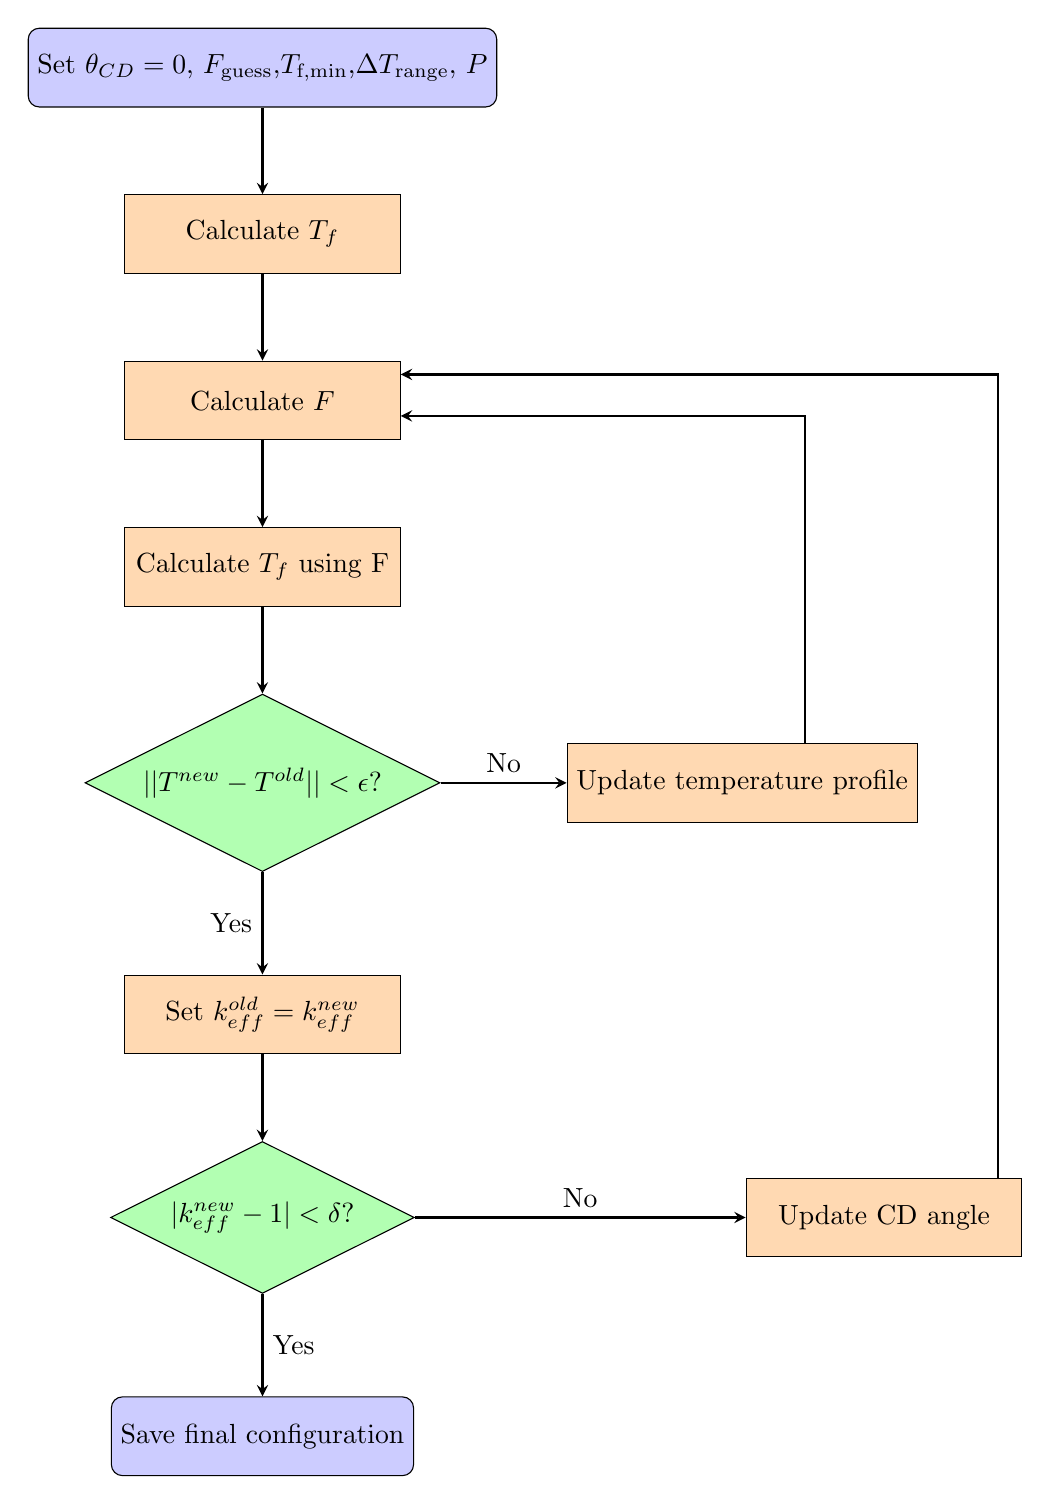
\begin{tikzpicture}[node distance=1.1cm and 1.6cm]

% Nodi principali
\node (start) [startstop] {Set $\theta_{CD} = 0$, $F_{\text{guess}}$,$T_{\text{f,min}}$,$\Delta T_{\text{range}}$, $P$};
\node (calcT1) [process, below=of start] {Calculate $T_f$};

\node (calcF) [process, below=of calcT1] {Calculate $F$};

\node (calcT2) [process, below=of calcF] {Calculate $T_f$ using F};


\node (tempConv) [decision, below=of calcT2] {$||T^{new} - T^{old}|| < \epsilon$?};
\node (updateT) [process, right=of tempConv, xshift=0.001cm] {Update temperature profile};
\node (returnTempLoop) [coordinate, above=of updateT, yshift=1cm] {};

\node (keffUpdate) [process, below=of tempConv, yshift=-0.2cm] {Set $k_{eff}^{old} = k_{eff}^{new}$};
\node (critConv) [decision, below=of keffUpdate] {$|k_{eff}^{new} - 1| < \delta$?};
\node (updateCD) [process, right=of critConv, xshift=2.6cm] {Update CD angle};
\node (end) [startstop, below=of critConv, yshift=-0.2cm] {Save final configuration};

% Flussi
\draw [arrow] (start) -- (calcT1);
\draw [arrow] (calcT1) -- (calcF);
\draw [arrow] (calcF) -- (calcT2);
\draw [arrow] (calcT2) -- (tempConv);

% Ciclo temperatura
\draw [arrow] (tempConv) -- node[above] {No} (updateT);
\draw [arrow] (updateT.north) ++(0.8,0) |- ([yshift=-20pt]calcF.north east);


% Dopo convergenza temperatura
\draw [arrow] (tempConv) -- node[left] {Yes} (keffUpdate);
\draw [arrow] (keffUpdate) -- (critConv);

% Ciclo esterno CD
\draw [arrow] (critConv) -- node[above] {No} (updateCD);
% \draw [arrow] (updateCD) |- (calcF);
\draw [arrow] (critConv) -- node[right] {Yes} (end);
\draw [arrow] (updateCD.north)  ++(1.45,0) |- ([yshift=-5pt]calcF.north east);

\end{tikzpicture}
}
\caption{Improved criticality search algorithm with unified loop returning to power distribution calculation.}
\label{fig:crit_search_unified_loop}
\end{figure}

\subsection{Error metrics}

In the results section, some test cases will be used to quantify the accuracy between the results obtained using the fission matrix method and a reference Serpent2 model. Two main parameters will be compared: the $k_{eff}$ and the neutron fission source ($\nu\Sigma_f\phi$ or $F$). The error displayed for the eigenvalue in the result section is defined in \Cref{eq:keff_err}. While \Cref{eq:fission_source_RMS_err} and \ \Cref{eq:fission_source_rel_err}, are used to account for the local and global error introduced by the fission matrix method for the neutron fission source, respectively. To quickly and easily double check the consistency of the fission source results, each Serpent2 reference case was run three separate times, using different random seeds for each run. For every simulation, the Root Mean Square Error (RMSE) of the fission source distribution was calculated, in order to assess how the uncertainty estimation varies depending on the random seed.

The comparison among the three sets of results revealed that the differences are negligible, and all outcomes are fully consistent with one another. This indicates that the stochastic variability introduced by the random seed has little to no impact on the reliability of the fission source estimation, and confirms the robustness of the results.   

\begin{equation}
    \Delta k_{eff} = k^{inter}_{eff} - k^{MC}_{eff}  \text{ (pcm)}
\label{eq:keff_err}
\end{equation}


\begin{equation}
    \text{e} = \frac{F_i^{inter}-F_i^{MC}}{F_i^{MC}} \cdot 100 \text{ (\%)}
\label{eq:fission_source_rel_err}
\end{equation}


\begin{equation}
    \text{RMSE}  = \sqrt{\frac{1}{N} \sum_i^N e_i^2 } \text{ (\%)}
\label{eq:fission_source_RMS_err}
\end{equation}



.
\section{Results and discussion}

\subsection{Database selection}

To ensure the accuracy of results while minimizing computational resources, we progressively increase the number of data points in our database. We start with a smaller dataset and then evaluate its sufficiency by reproducing a set of reference test cases. If the Root Mean Square Error (RMSE) of the $k_{eff}$ for these tests does not fall within the acceptable limit (below 2$\sigma_{k_{eff}}$ $k_{eff}$), we then increase the number of data points, moving to a larger database. 

The test cases used are the same for all databases and are selected by taking the midpoint between two neighboring points of the the most refined one. The author acknowledges the existence of more rigorous approaches (e.g., Smolyak grids); however, a simplified strategy was intentionally adopted to maintain clarity and ease of implementation.

In \Cref{fig:linear_interpolation_improvment_changing_database} is shown the $\Delta k_{eff}$ between the interpolated fission matrix and the Serpent2 reference value by changing the database used for the interpolation. As can be seen, only with the third database the error of most of the simulation reaches a value comparable with the Serpent2 uncertainty. More results information are listed in \Cref{tab:table_delta_k_linear}.


\begin{figure}[h!]
\centering
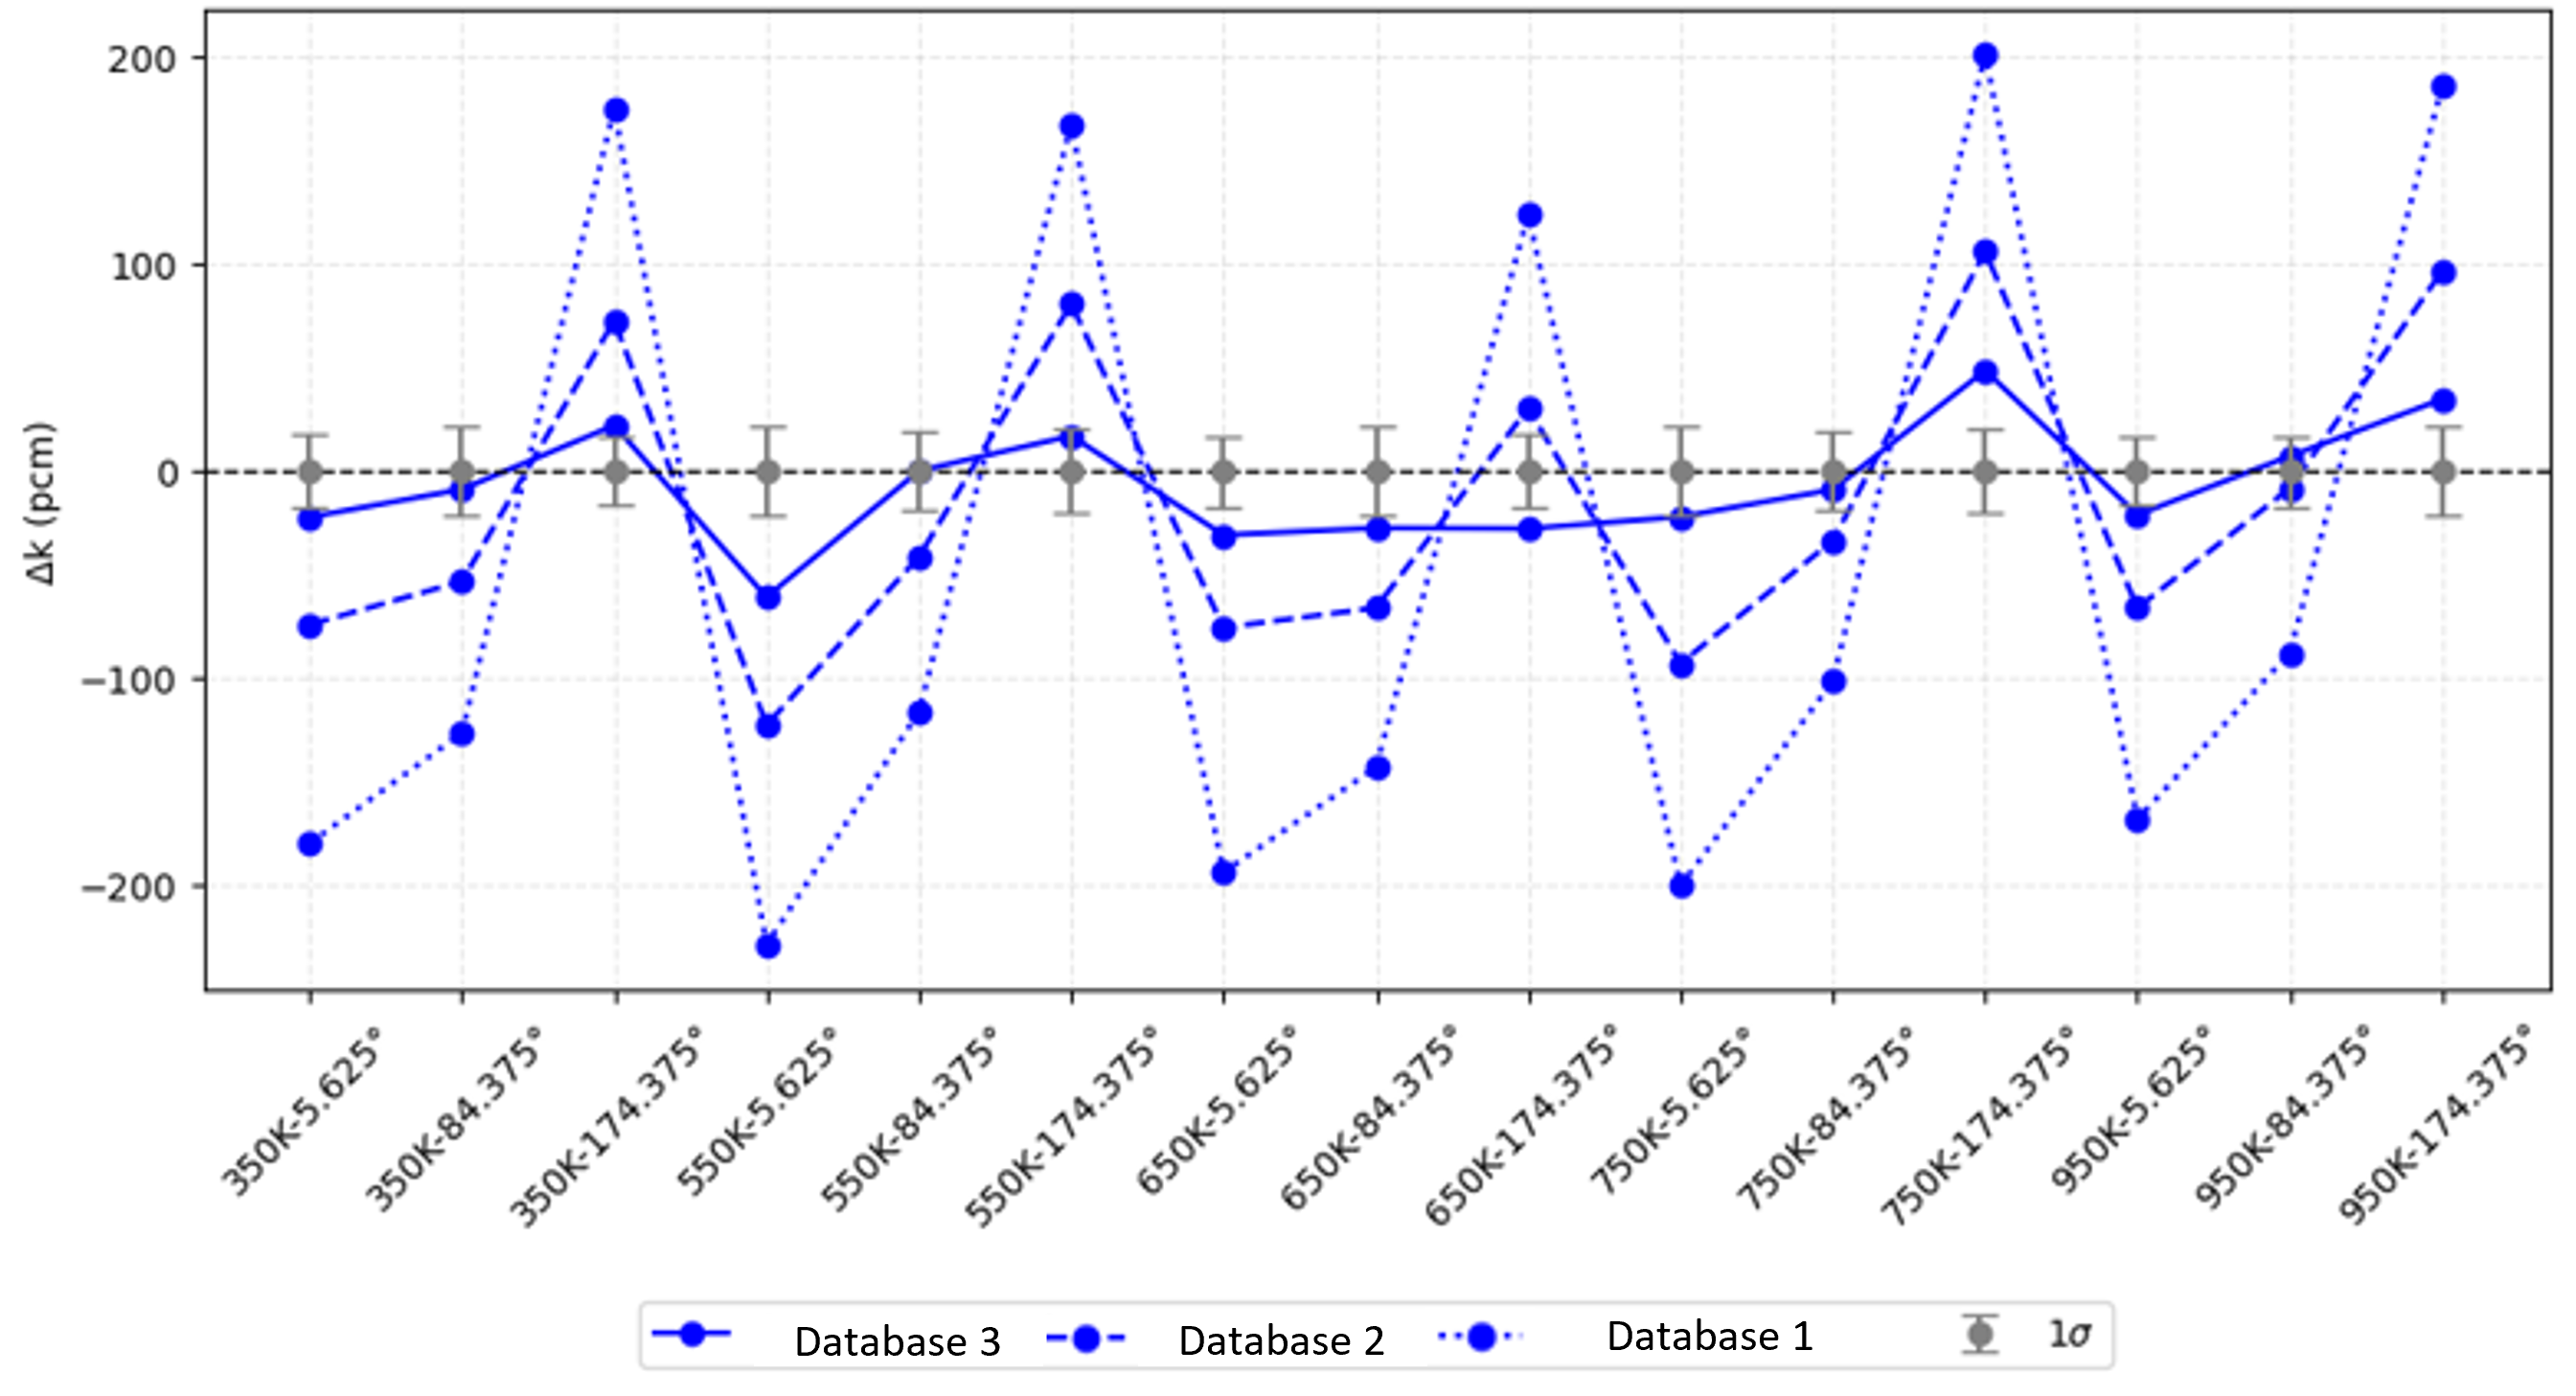
\includegraphics[scale=0.5]{images/linear_interpolation_improvment_changing_database.png}  % Modifica scale o usa width se serve
\caption{$\Delta k_{eff}$ using linear interpolation and varying the database.}
\label{fig:linear_interpolation_improvment_changing_database}
\end{figure}


\begin{table}[h!]
\centering
\caption{Interpolation errors for different databases using the linear method.}
\label{tab:table_delta_k_linear}
\begin{tabular}{lccccc}
\cline{2-6}
           & \multicolumn{3}{c}{$\Delta k_{eff}$ (pcm)} & RMSE - $\nu\Sigma_f\phi$ (\%)   & $max(\left|e \right|)$   \\ \cline{2-6} 
           & Min                & Max                & RMSE               &          & RMSE             \\ \hline
Database 1 & 0.089              & 61.01              & 28.506             & 0.82 &  1.2                    \\ \hline
Database 2 & 8.44               & 122.76             & 74.24              & 1.1  &  1.6            \\ \hline
Database 3 & 87.866             & 228.73             & 164.85             & 1.12 &  2.4              \\ \hline
\end{tabular}
\end{table}




In total, eight fuel temperature and seventeen CDs angle values are considered in the final database. In \Cref{fig:databases} the points of the three databases are reported along with the test points.     


\begin{figure}[h!]
\centering
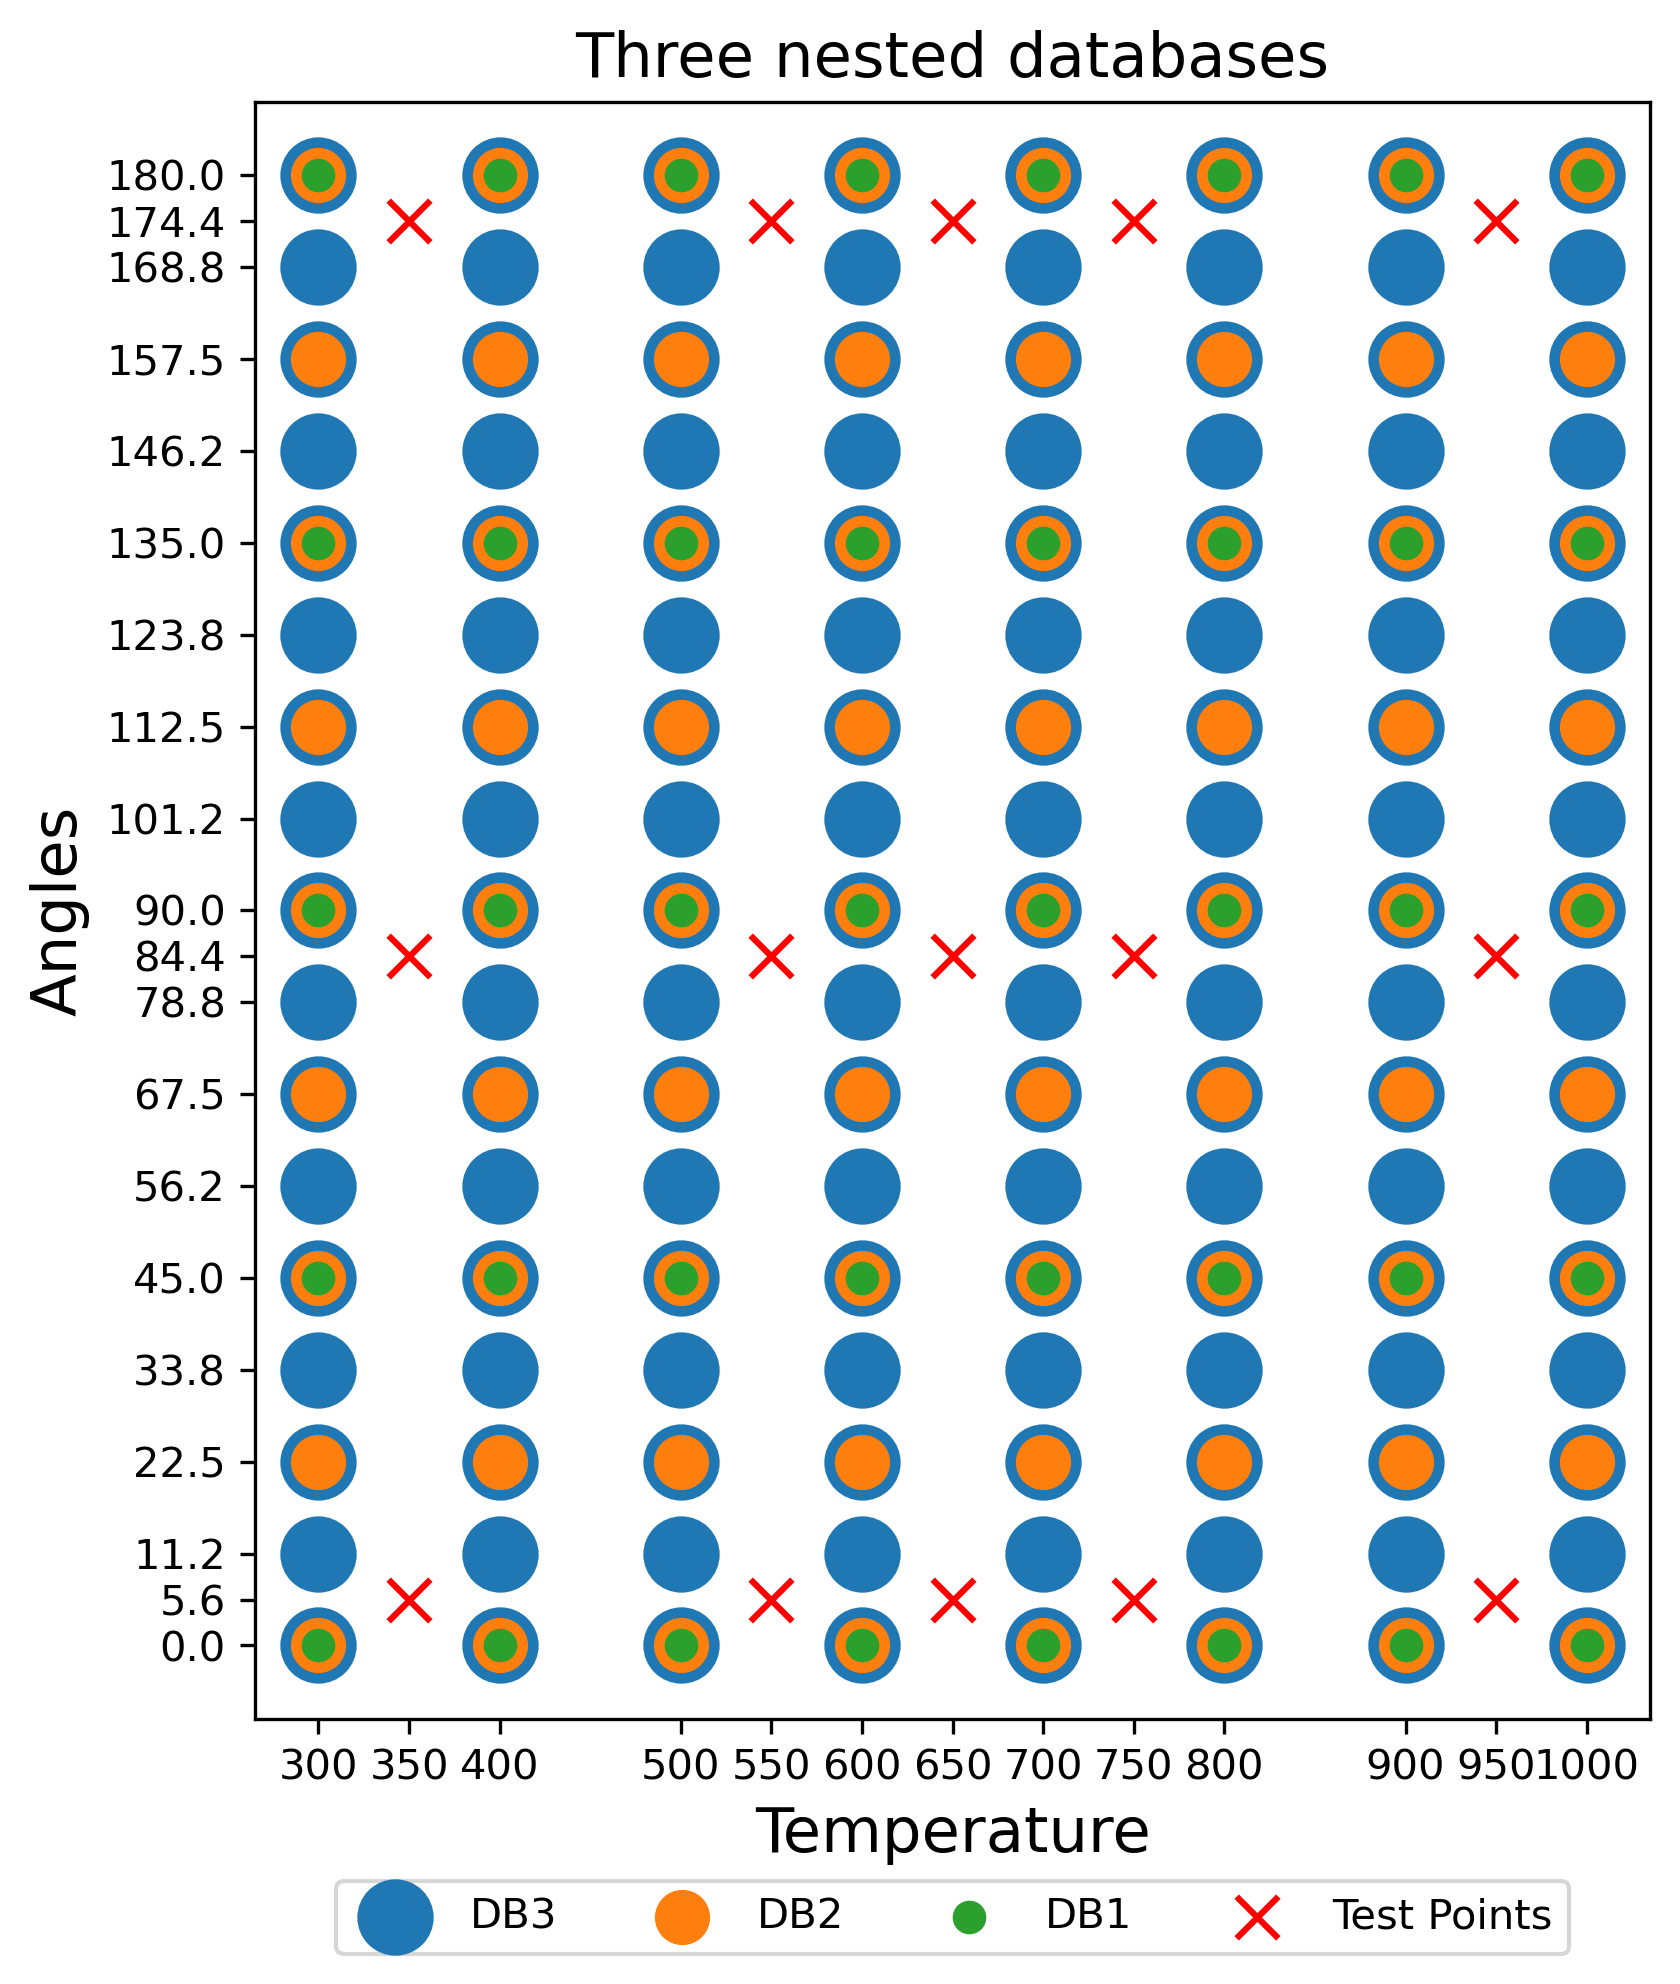
\includegraphics[scale=0.45]{images/nested_databases.png}  % Modifica scale o usa width se serve
\caption{Databases point distribution. The green points are the data of the first and less dense database, the orange one is the intermediate one, and the blue points is the finest database available. The red crosses represent the testing cases.}
\label{fig:databases}
\end{figure}

In \Cref{fig:databases}, the data distribution for the various databases is schematized. As the figure illustrates, the primary difference among the three nested databases lies in the number of points considered for the control drums angle, which ranges from 0° to 180° due to the symmetry of the effect beyond this angle. The red crosses indicate the points used for the testing cases. 

The reason why only the number of control drum (CD) rotation angles increases between the different databases lies in the stronger and more nonlinear impact of CD rotation on the reactor’s reactivity and, consequently, on the values of the fission matrix; as observed also in \cite{Rau2021Proc}. In contrast, variations in fuel temperature tend to produce more gradual and linear effects on neutron behavior. (MAYBE HERE IT WOULD BE BETTER TO REPORT A $   k_{eff}$ VS CD angle PLOT AND $   k_{eff}$ VS $T_{fuel}$ TO SHOW THAT TEMPERATURE FEEDBCK IS LINEAR, WHILE CD INSERTION HAS A "S" CURVE).  





\subsection{Correction ratios tests}
 These simulations involve variations in both the temperature distribution and the control drum positions.

A representative subset of the test cases is presented and described in \cref{tab:cases_testing_cases_for_gradient_T}. These cases were selected to best illustrate the accuracy of the method in scenarios where a uniform temperature distribution is directly imposed, as well as to highlight how the accuracy may degrade when no correction factor is applied, particularly in configurations where the reflector temperature differs from that of the core.        


\begin{table}[h!]
\caption{Testing cases with temperature gradient fissile and non fissile assemblies.}
\centering
\begin{tabular}{llll}
\hline
       & $T_f$ & $T_r$ & $\theta$ \\ \hline
case 1 & 550K  & 300K  & 0°       \\ \hline
case 2 & 550K  & 300K  & 90°      \\ \hline
case 3 & 950K  & 300K  & 0°       \\ \hline
case 4 & 950K  & 300K  & 90°      \\ \hline
\end{tabular}
\label{tab:cases_testing_cases_for_gradient_T}
\end{table}

These four distinct test cases, are specifically designed to analyze the performance of the proposed correction methods under varying conditions of temperature gradients. By examining scenarios with different fuel temperatures ($T_f$), reflector temperatures ($T_r$), and CD rotation angle ($\theta$), we aim to comprehensively assess how effectively the correction ratio. A temperature distribution sample of the case where $T_f \neq T_r$ is shown in \cref{fig:temperature_distribution_example_different_T_fuel_reflector}.

\begin{figure}[]
\centering

\includegraphics[scale=0.5]{images/grad_temp_core_reflector.png}  % Modifica scale o usa width se serve
\caption{Temperature distribution sample with different temperature of the fuel (red)  and reflector (blue).}
\label{fig:temperature_distribution_example_different_T_fuel_reflector}
\end{figure}

The results are reported in \cref{tab:cases_testing_cases_for_gradient_T2}. Where $\Delta{k_{eff}}$, the maximum absolute value of e and the RMSE are reported, using different correction ratios (CRs). In \cref{fig:Tf_550_Tr_300_4_plots} and \cref{fig:Tf_550_Tr_300_CD_90_4_plots} Case 1 and Case 2, relative uncertainty, fission source obtained with the fission matrix method, the ratio between the e values and the corresponding relative uncertainty of both non-corrected and corrected cases, are displayed. Only the corrected cases using \cref{eq:correction_ratio_2} is shown. 

\begin{table}[h!]
\caption{Testing cases with different uniform $T_f$ and $T_r$ and CD position error.}
\centering
\begin{tabular}{llcccc}
\cline{3-6}
&                                                  & Case 1 & Case 2 & Case 3 & Case 4 \\ \hline
$\sigma_{k_{eff}}$                                      & \multicolumn{1}{l|}{CR}                            & 18     & 17     & 19     & 18     \\ \hline
\multirow{3}{*}{$\Delta k_{eff}$ (pcm)} & \multicolumn{1}{l|}{$1$}       & -111   & -176   & -352   & -415   \\
& \multicolumn{1}{l|}{$r_{ij}$ def.1}         & -2     & -131   & 5      & -305   \\
& \multicolumn{1}{l|}{$r_{ij}$ def.2} & -     & 4      & -      & 14     \\ \hline
\multirow{3}{*}{max($|e|$) (\%)}                               & \multicolumn{1}{l|}{$1$}     & 4.6    & 6.5    & 6.2    & 7.6    \\
& \multicolumn{1}{l|}{$r_{ij}$ def.1}         & -2     & -131   & 5      & -305   \\
& \multicolumn{1}{l|}{$r_{ij}$ def.2} & -    & 0.53   & -   & 0.5    \\ \hline
\multirow{3}{*}{RMSE (\%)}        & \multicolumn{1}{l|}{$1$}       & 2.0    & 5.4    & 4.6    & 5.2    \\
& \multicolumn{1}{l|}{$r_{ij}$ def.1}         & -2     & -131   & 5      & -305   \\
& \multicolumn{1}{l|}{$r_{ij}$ def.2} & -    & 0.4    & -    & -    \\ \hline
\end{tabular}
\label{tab:cases_testing_cases_for_gradient_T2}
\end{table}




\begin{figure}[h!]
\centering
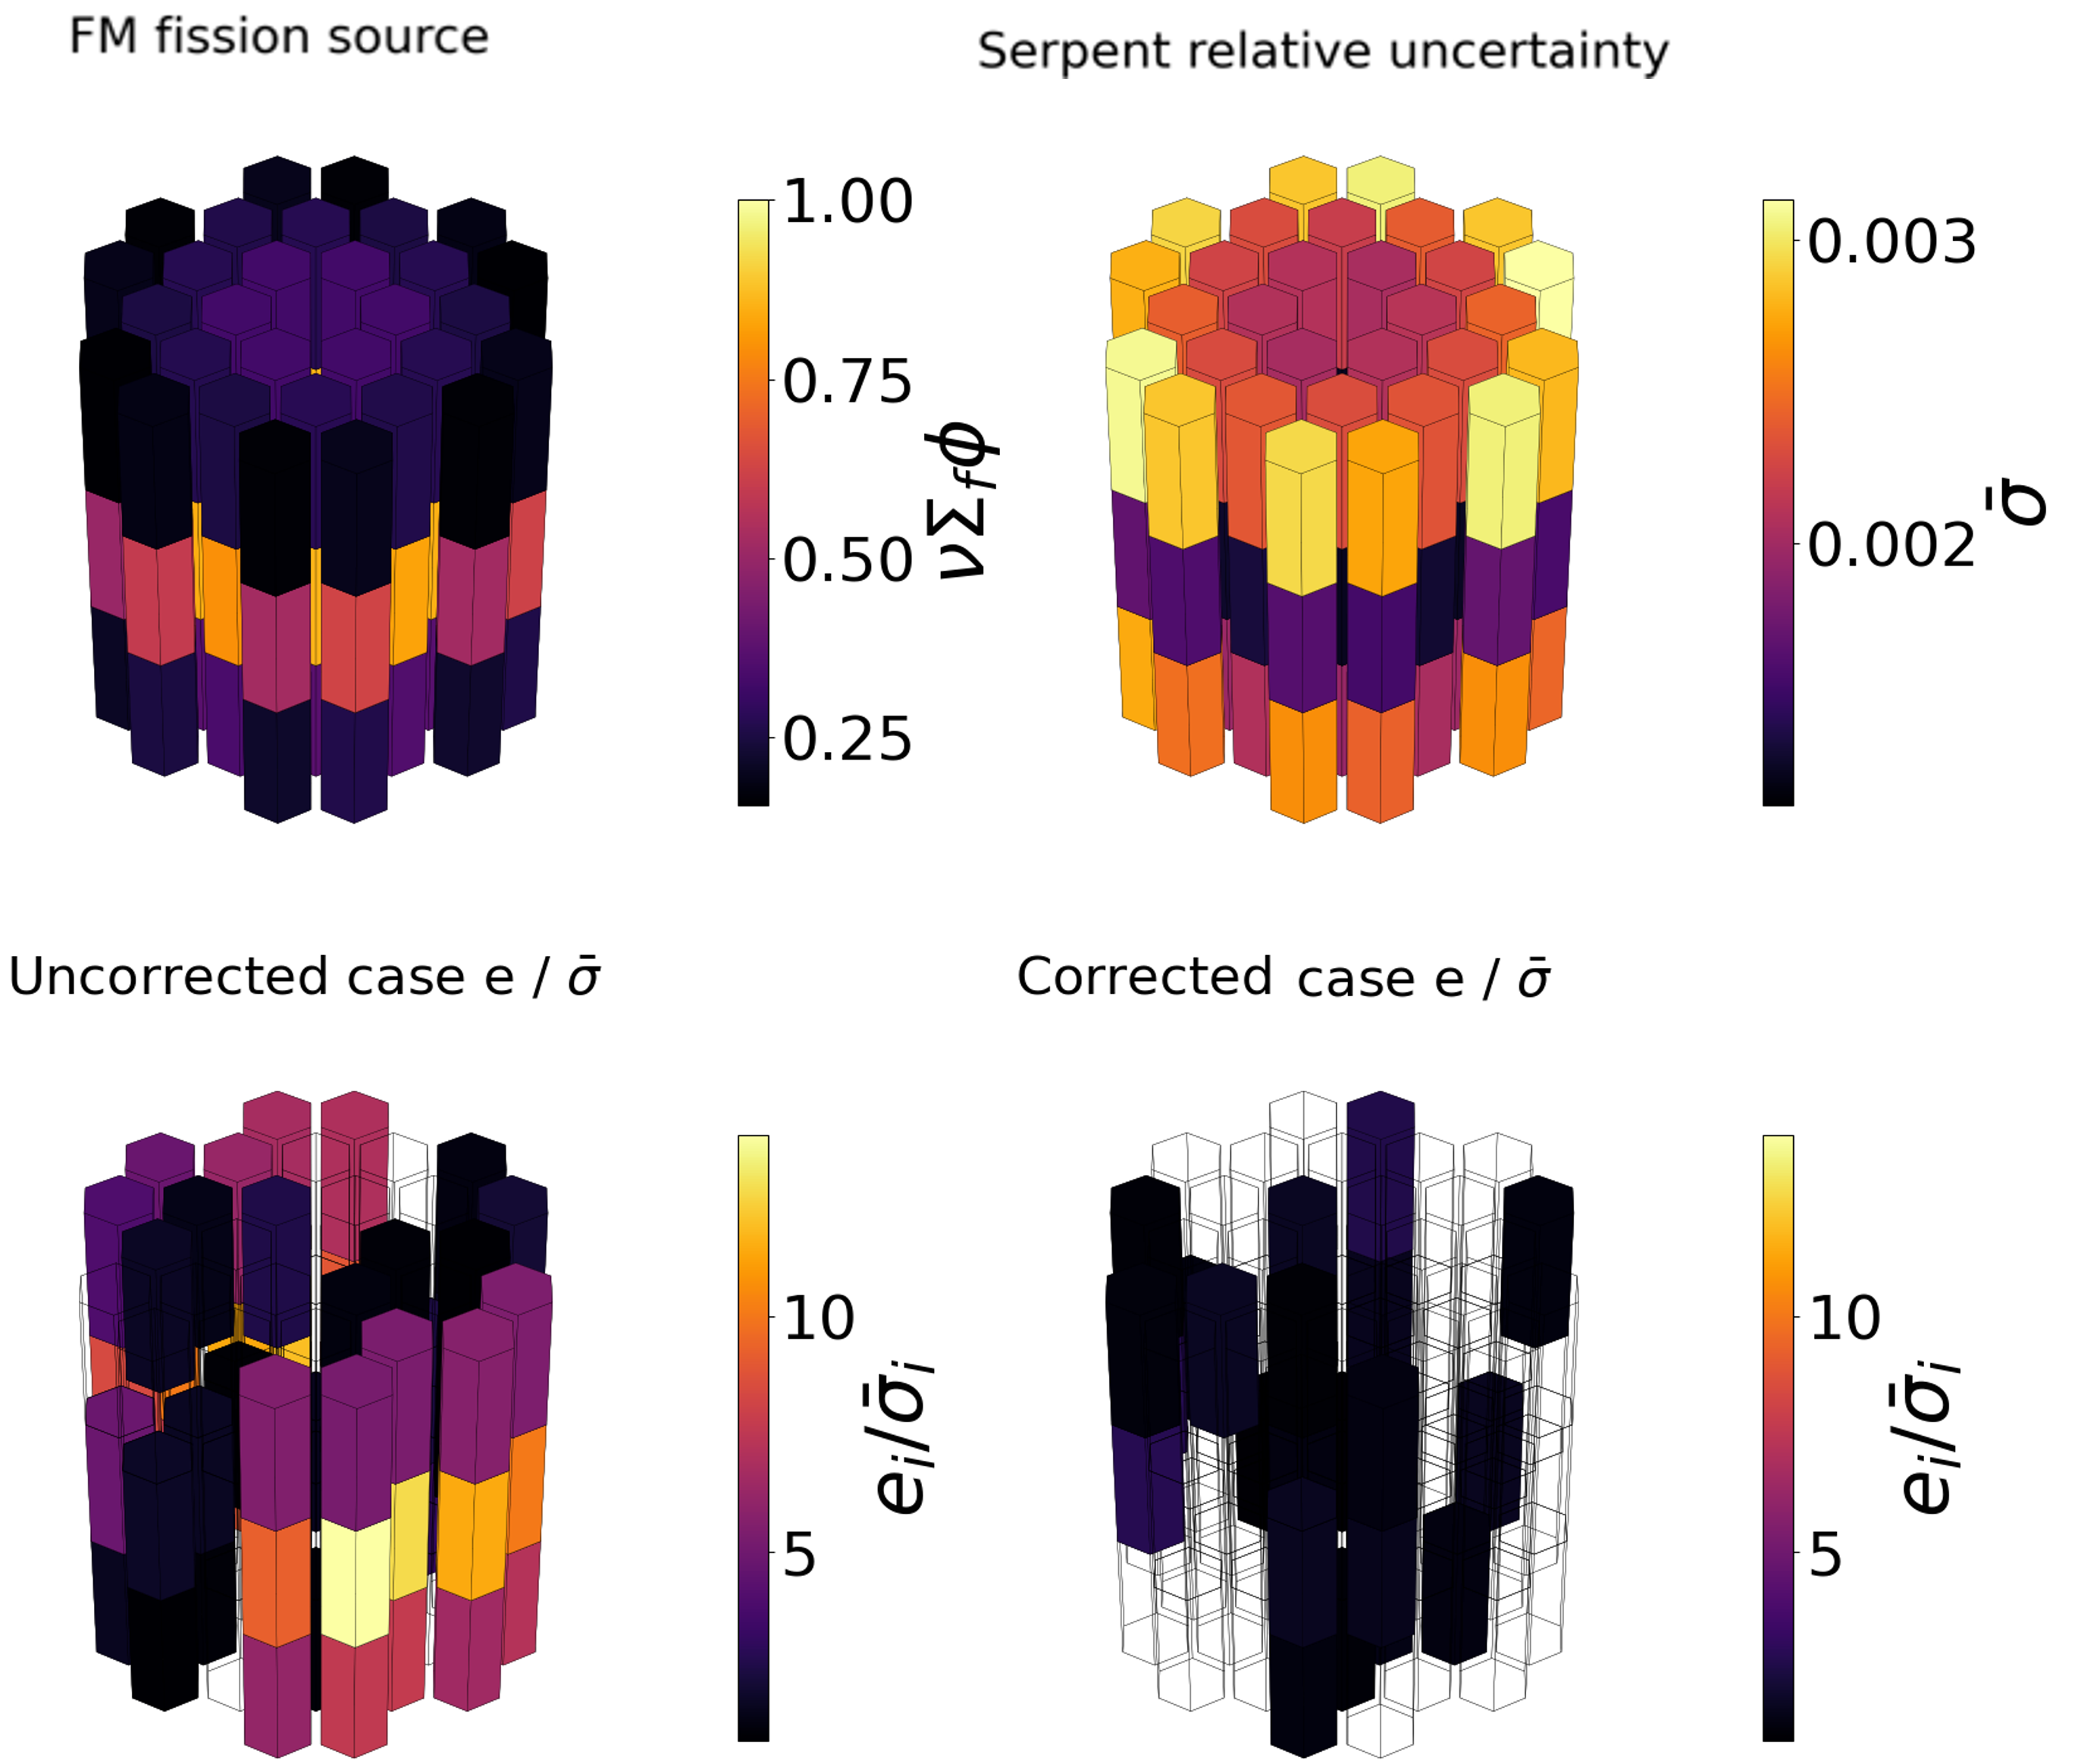
\includegraphics[scale=0.60]{images/Tf_550_Tr_300_4_plots.png}  % Modifica scale o usa width se serve
\caption{Case 1 of \cref{tab:cases_testing_cases_for_gradient_T}. The corrected-case refers to the one using \cref{eq:correction_ratio_2} }
\label{fig:Tf_550_Tr_300_4_plots}
\end{figure}

\begin{figure}[h!]
\centering
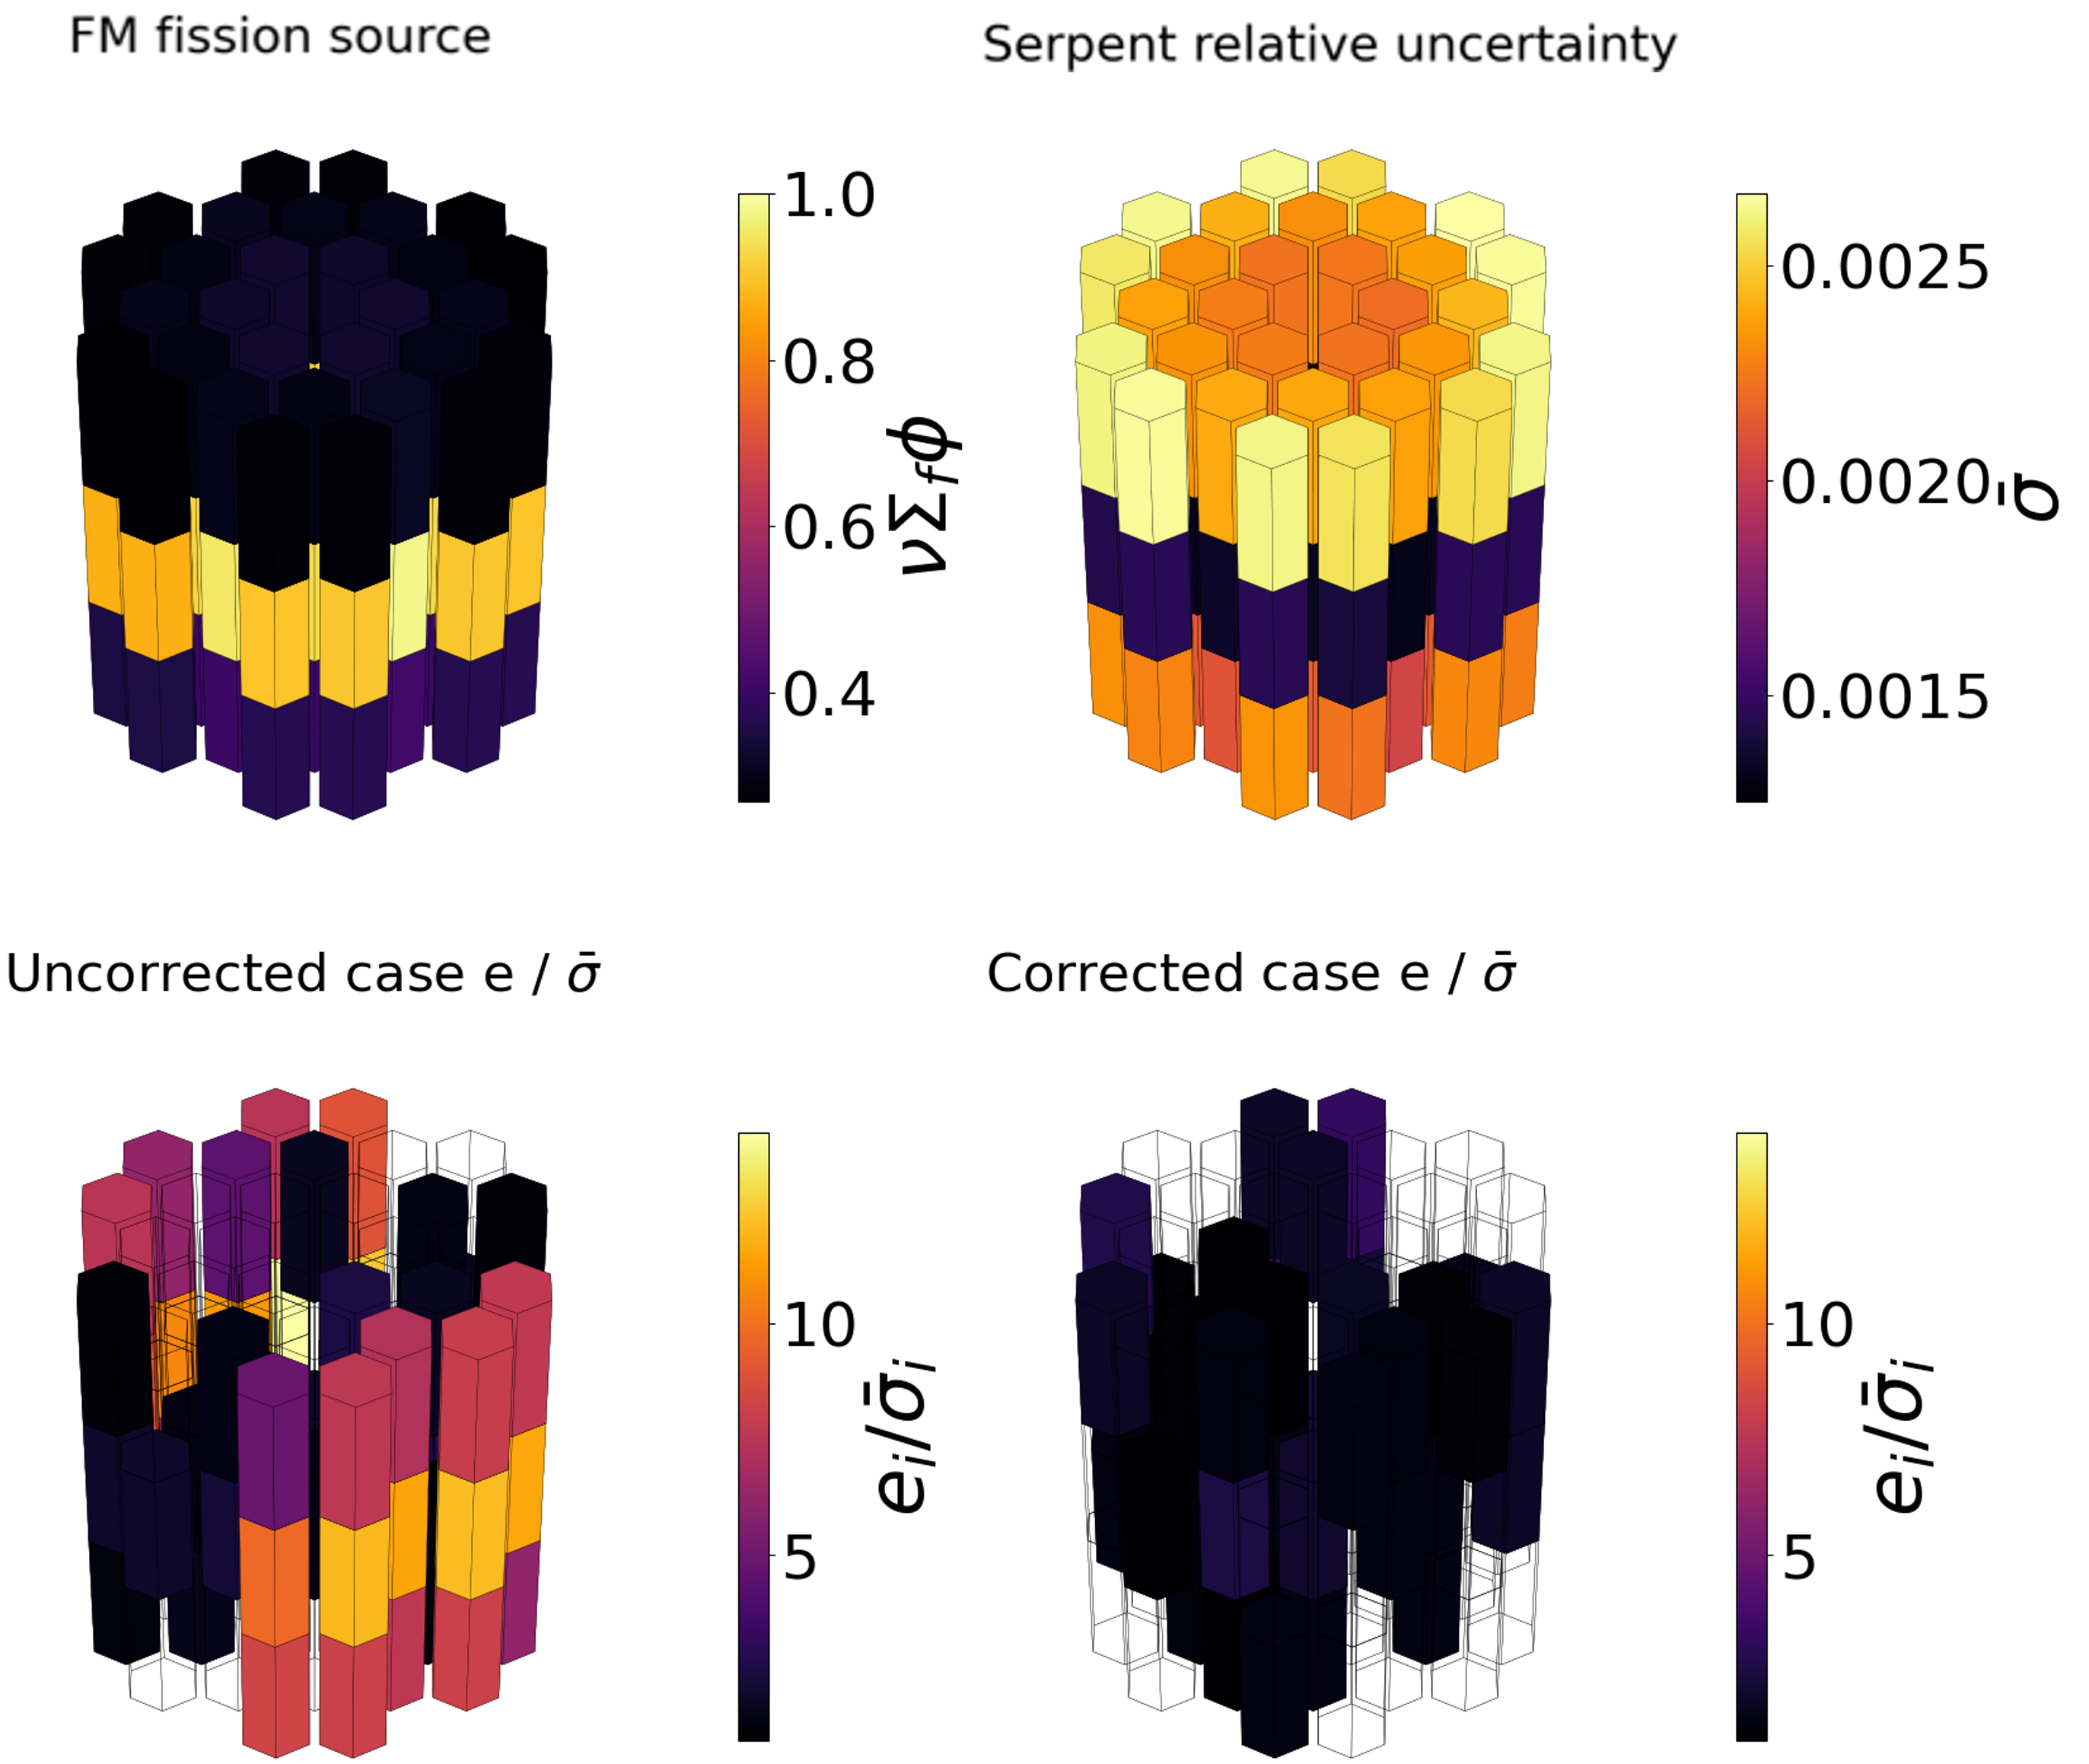
\includegraphics[scale=0.60]{images/Tf_550_Tr_300_CD_90_4_plots.png}  % Modifica scale o usa width se serve
\caption{Case 2 of \cref{tab:cases_testing_cases_for_gradient_T}. The corrected-case refers to the one using \cref{eq:correction_ratio_2} }
\label{fig:Tf_550_Tr_300_CD_90_4_plots}
\end{figure}


The results using the correction ratio defined in \cref{eq:correction_ratio_2} are  under the Serpent2 uncertainty values. 


\subsection{Core temperature distribution tests}
To better analyze how the method performs when a non-uniform and non-symmetric temperature distribution is used, three more test cases are reported. The first one (case 5) uses a non-uniform symmetric $T_f$ distribution, where the second one (case 6) uses a non-uniform, non-symmetric distribution, while the third one (case 7) uses a realistic temperature distribution relying on \cref{eq:correction_power_temperature}. 
In case \cref{fig:cases_5_6_7_temperature_distributions} the temperature distributions of the three new cases are shown. 


\begin{figure}[h!]
\centering
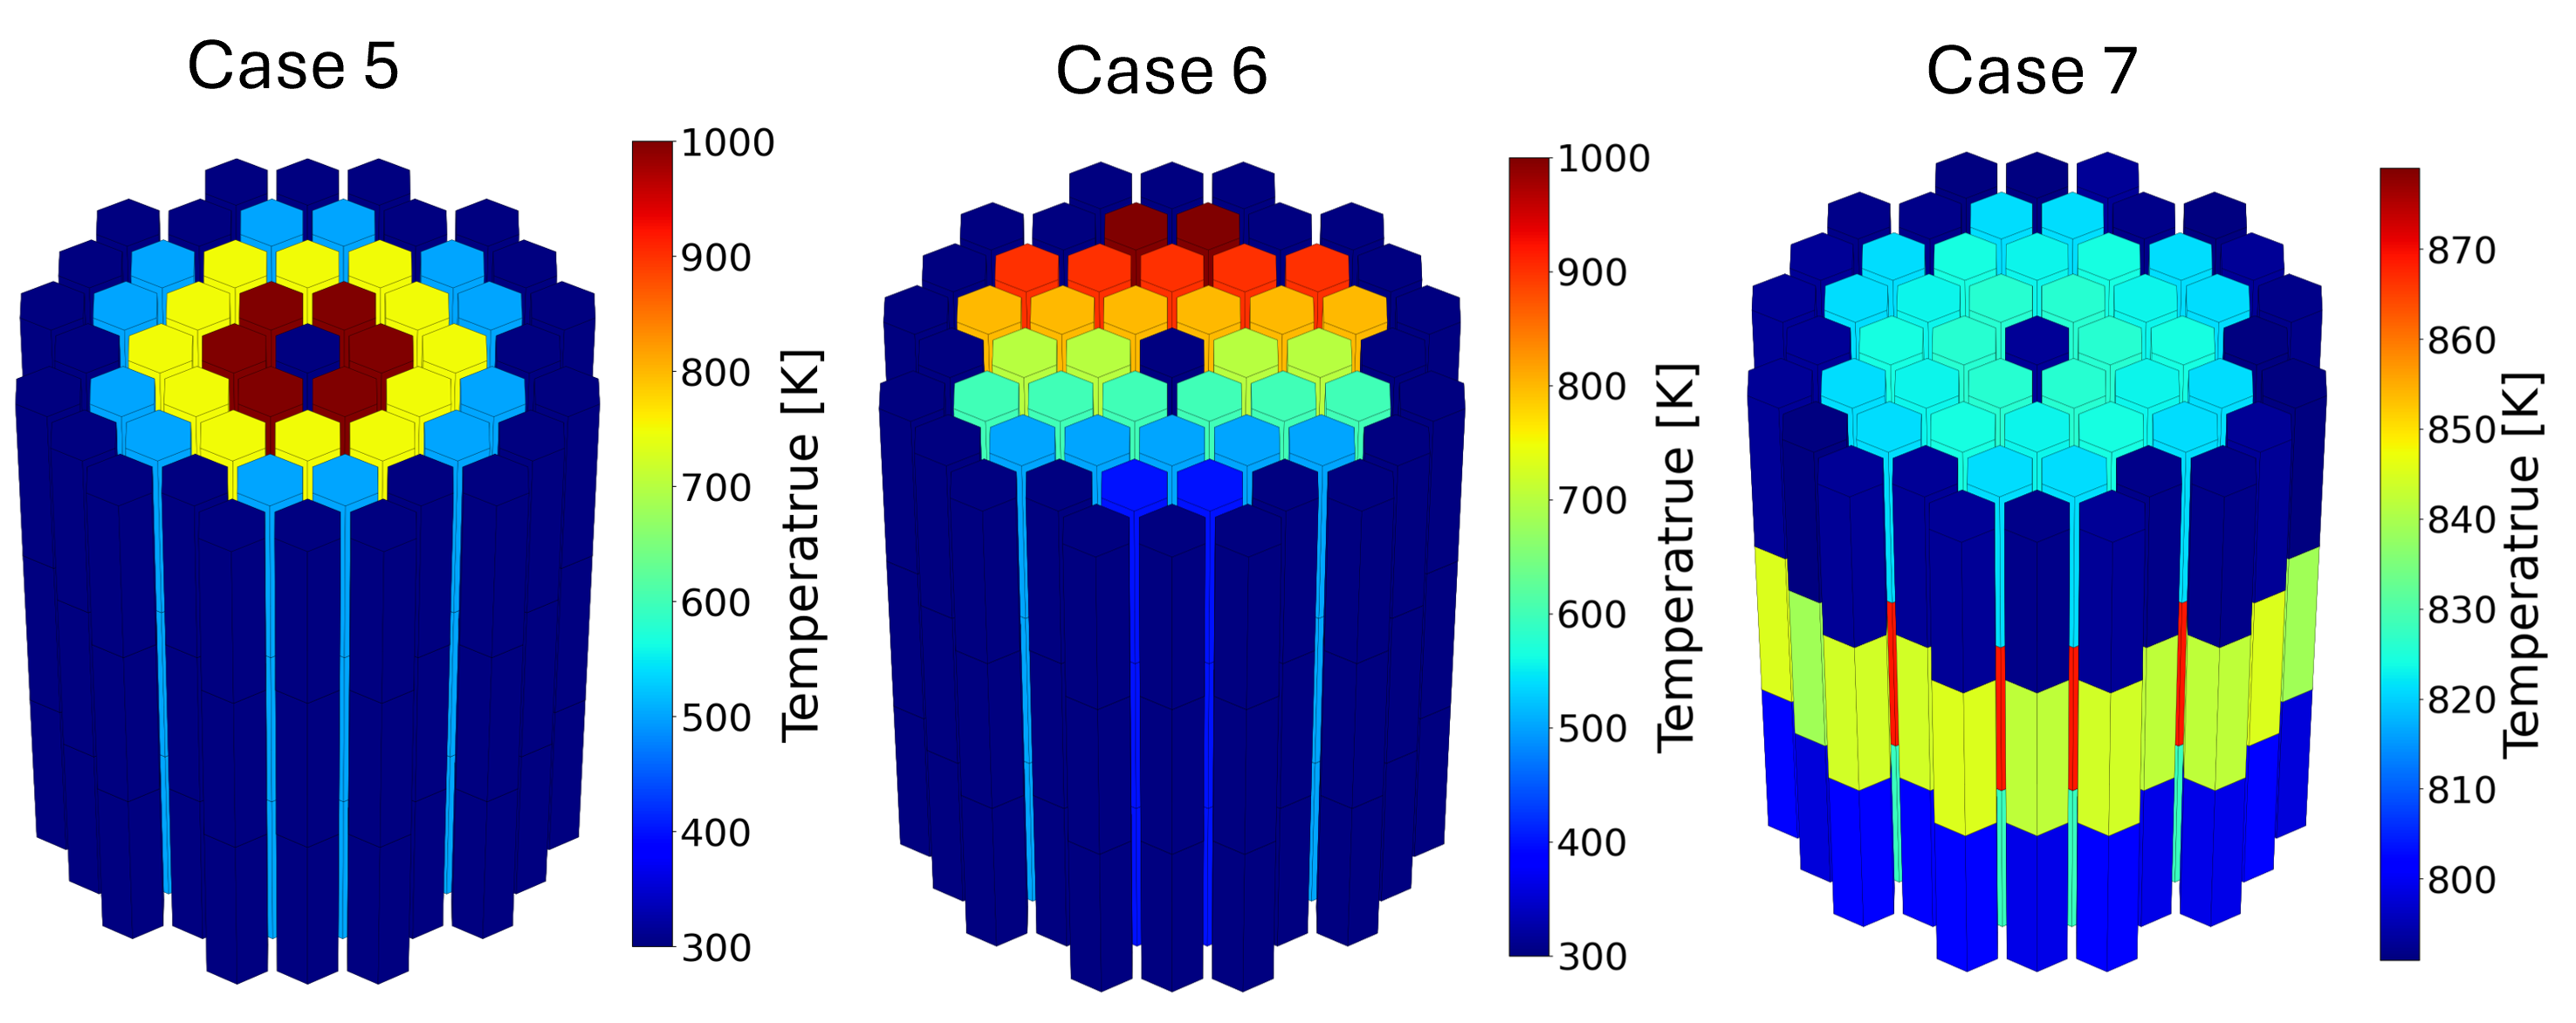
\includegraphics[scale=0.6]{images/cases_5_6_7_temperature_distributions.png}  % Modifica scale o usa width se serve
\caption{Case 5,6,7 temperature distributions.}
\label{fig:cases_5_6_7_temperature_distributions}
\end{figure}

In Case 5, three different temperature values are defined over the three rings of fuel of the system. The temperature decreases from the center towards the outer ring. The reflector temperature is set to 300 K, the outer ring is 500 K, the middle one 750 K and the inner one 1000 K.
In Case 6, the temperature of the fuel increases linearly along the y-direction, starting from 350 K to 1000 K, while the reflector temperature is set to 300 K.
In Case 7 \cref{eq:correction_power_temperature} is used to define a temperature distribution proportional to the fission source, hence, to the power distribution of the system. As described previously, \cref{eq:correction_power_temperature}, requires the set of the $\Delta T_{range}$ and $T_{f,min}$ parameter. Moreover, since, the corresponding fission source of the temperature distribution is not known apriori, the temperature has to be updated iteratively by changing the fission source distribution with the new one, obtained by the previous evaluated fuel temperature distribution. 
In Case 7 the considered power is equal to 2 MW (equal to the nominal power), and  $T_{range}$ = 100 K and $T_{f,min}$ = 800 K. These parameters have been defined by considering the temperature distribution of a high-fidelity simulation using Griffin of the same model at nominal power with extracted CDs. 

\begin{figure}[h!]
\FloatBarrier
\centering
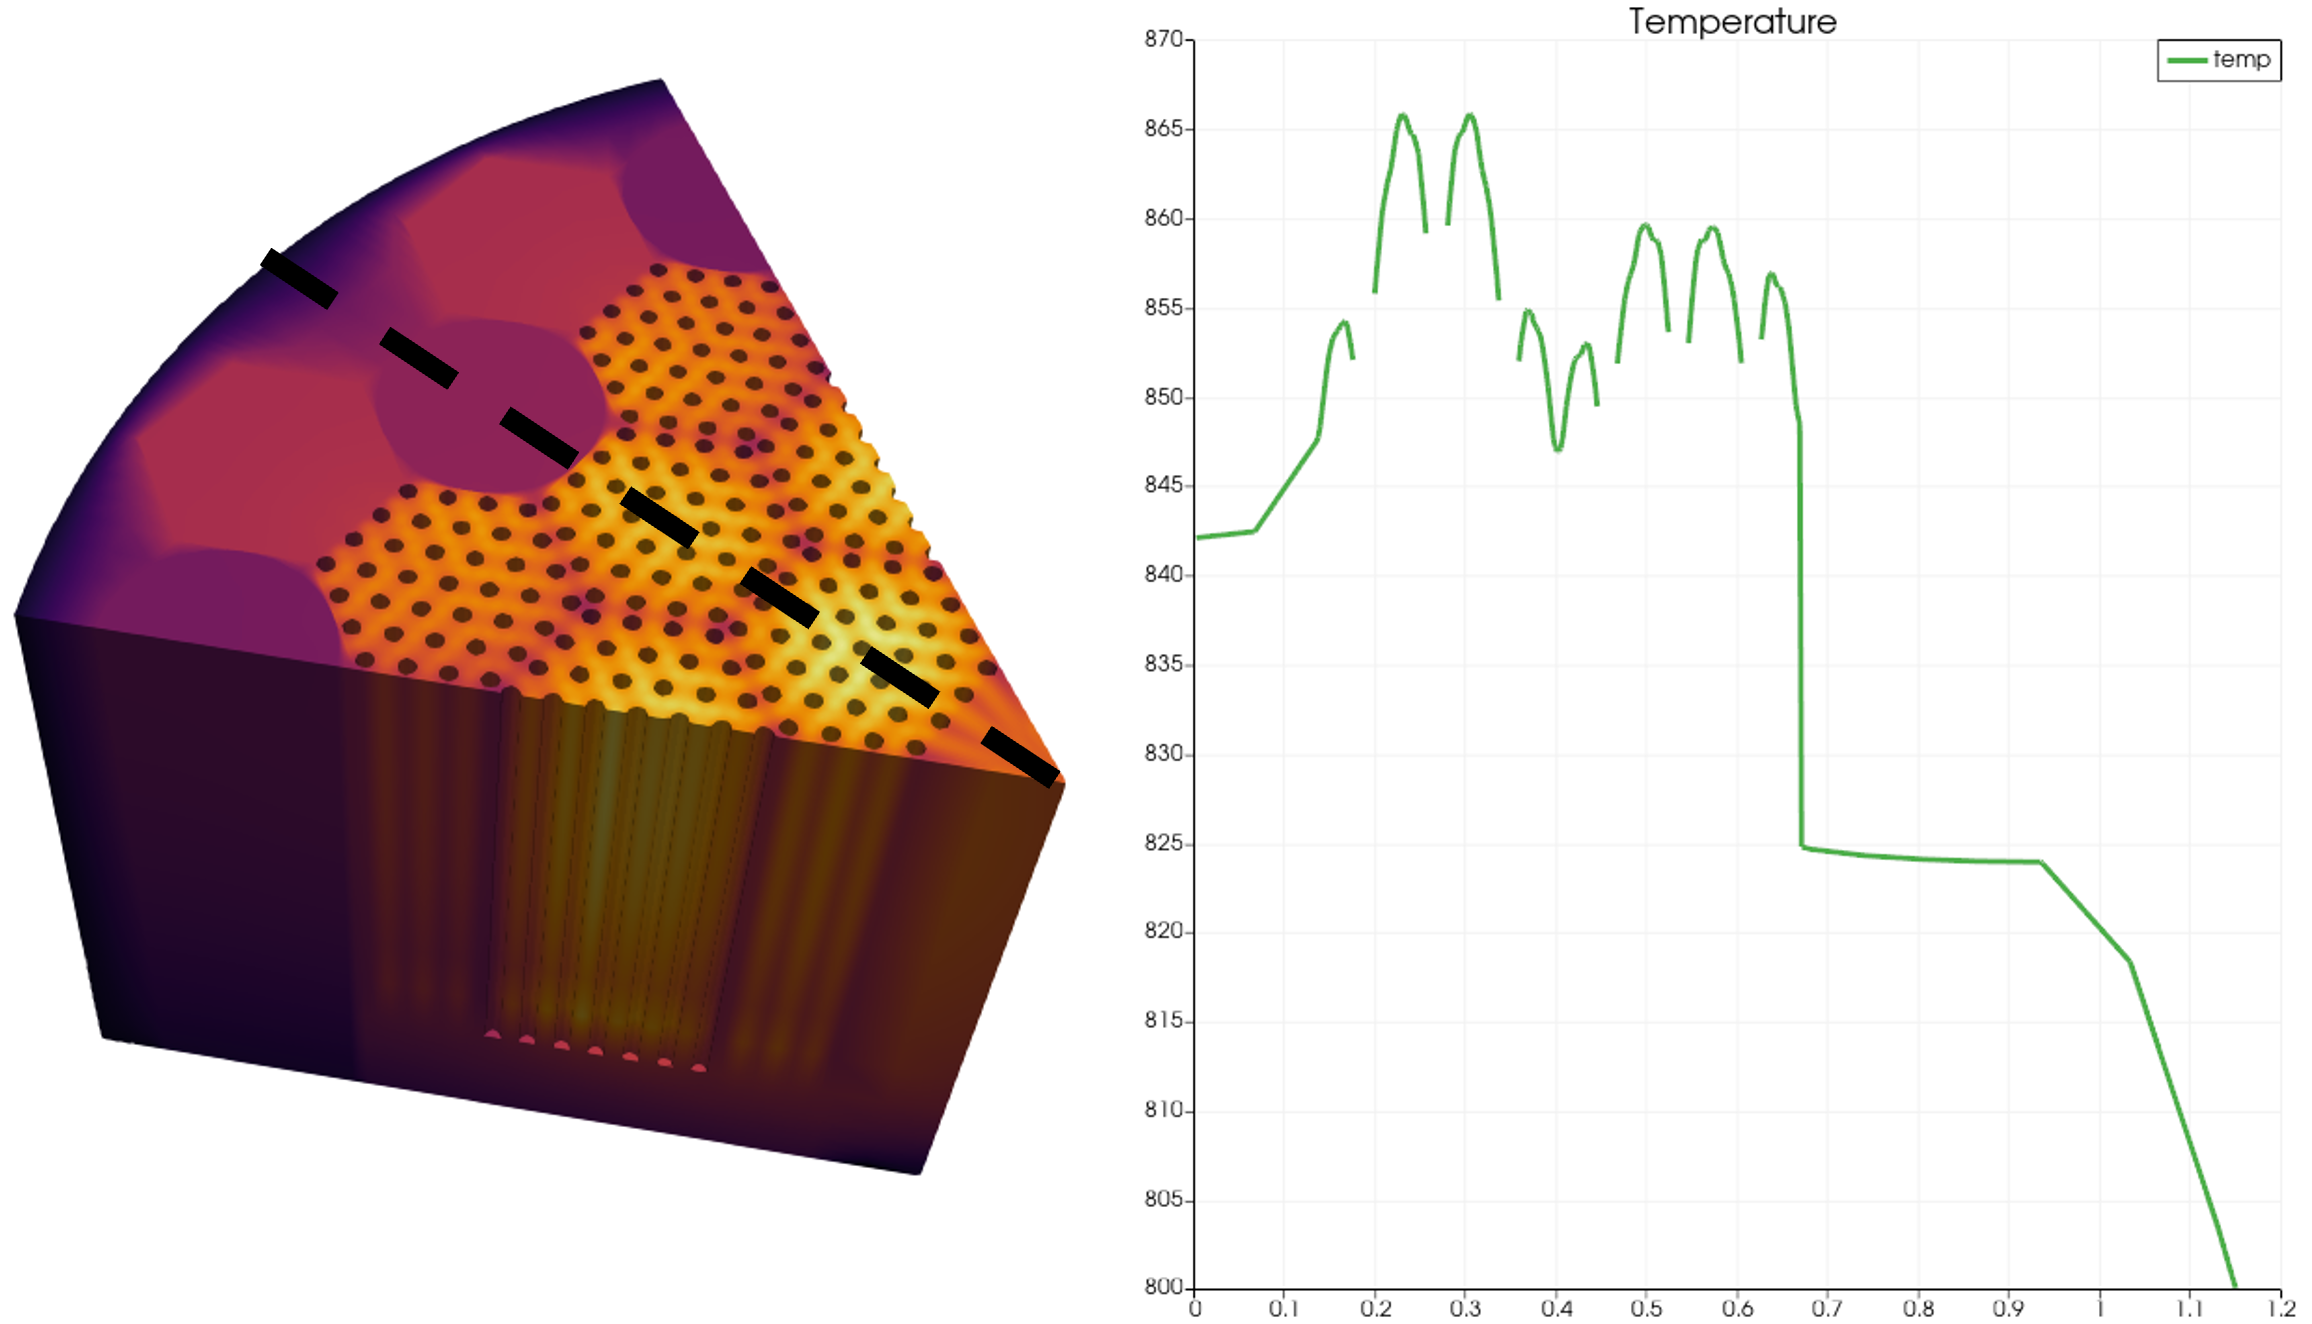
\includegraphics[scale=0.65]{images/realistic_temperature_desing_cenrtal_line_plot_horizontal.png}  % Modifica scale o usa width se serve
\caption{Temperature distribution example with different temperature of the fuel (red)  and reflector (blue).}
\label{fig:comparison_tetst_cases_wo_and_w_correction_ratio1}
\end{figure}

The results of these additional cases are reported in \cref{tab:testing_cases_5_6_7} and \cref{fig:Tf_rings_case_5},\cref{fig:Tf_linear_case_6},\cref{fig:Tf_power_like_case_7}. 


\begin{table}[h!]
\FloatBarrier
\caption{Testing cases with different uniform $T_f$ and $T_r$ (CR = 1 and $r_{ij}$ def.2 only).}
\centering
\begin{tabular}{llccc}
\cline{3-5}
&                                                  & Case 5 & Case 6 & Case 7 \\ \hline
$\sigma_{k_{eff}}$ & \multicolumn{1}{l|}{CR}         &    16    &    21    & 18       \\ \hline
\multirow{2}{*}{$\Delta k_{eff}$ (pcm)}   
& \multicolumn{1}{l|}{$1$}               &  -102      & -201       &   -64     \\
& \multicolumn{1}{l|}{$r_{ij}$ def.2}    &   -62     &  3      &     -32   \\ \hline
\multirow{2}{*}{max($|e|$) (\%)}     
& \multicolumn{1}{l|}{$1$}               &    7.8    &   2.4     &    2.0    \\
& \multicolumn{1}{l|}{$r_{ij}$ def.2}    &    5.0   &   4.5     &     2.0   \\ \hline
\multirow{2}{*}{RMSE (\%)}         
& \multicolumn{1}{l|}{$1$}               &     4.0   &   3.2  &   0.7     \\
& \multicolumn{1}{l|}{$r_{ij}$ def.2}    &      2.1  &   1.8   &   0.6     \\ \hline
\end{tabular}
\label{tab:testing_cases_5_6_7}
\end{table}


\begin{figure}[h!]
\FloatBarrier
\centering
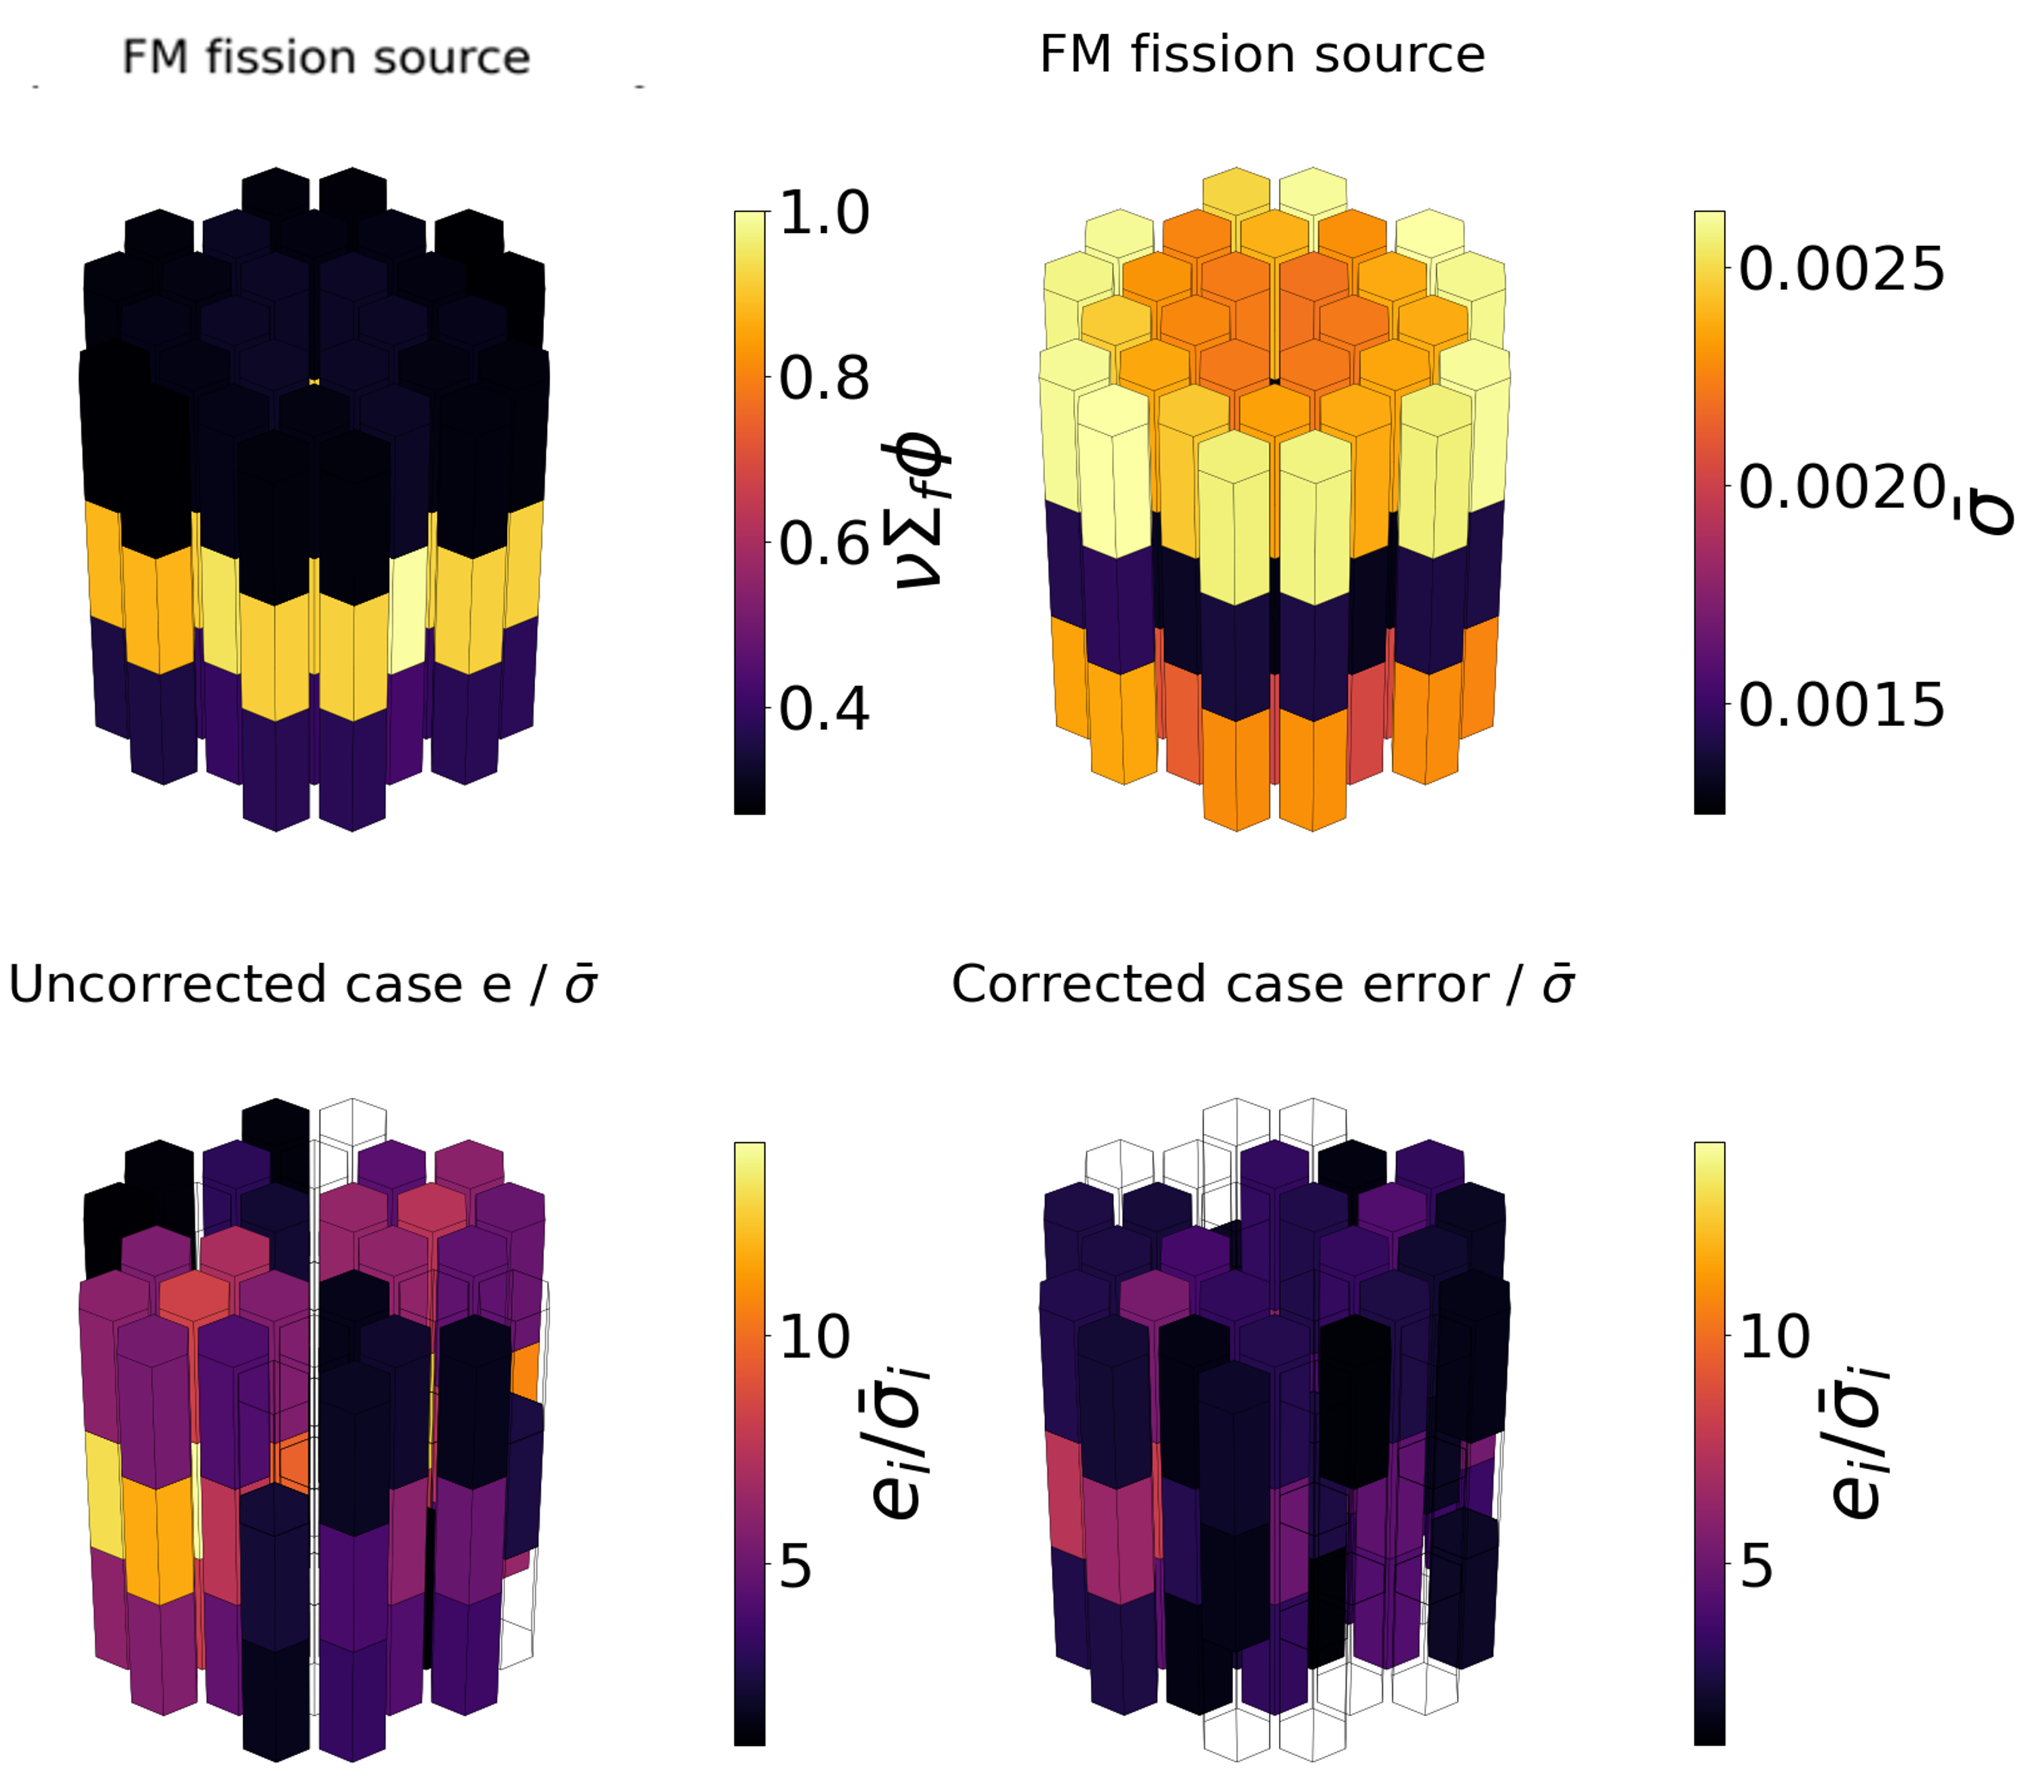
\includegraphics[scale=0.6]{images/Tf_rings_case_5.png}  % Modifica scale o usa width se serve
\caption{Case 5 of \cref{tab:testing_cases_5_6_7}. The corrected-case refers to the one using \cref{eq:correction_ratio_2} }
\label{fig:Tf_rings_case_5}
\end{figure}

\begin{figure}[h!]
\FloatBarrier
\centering
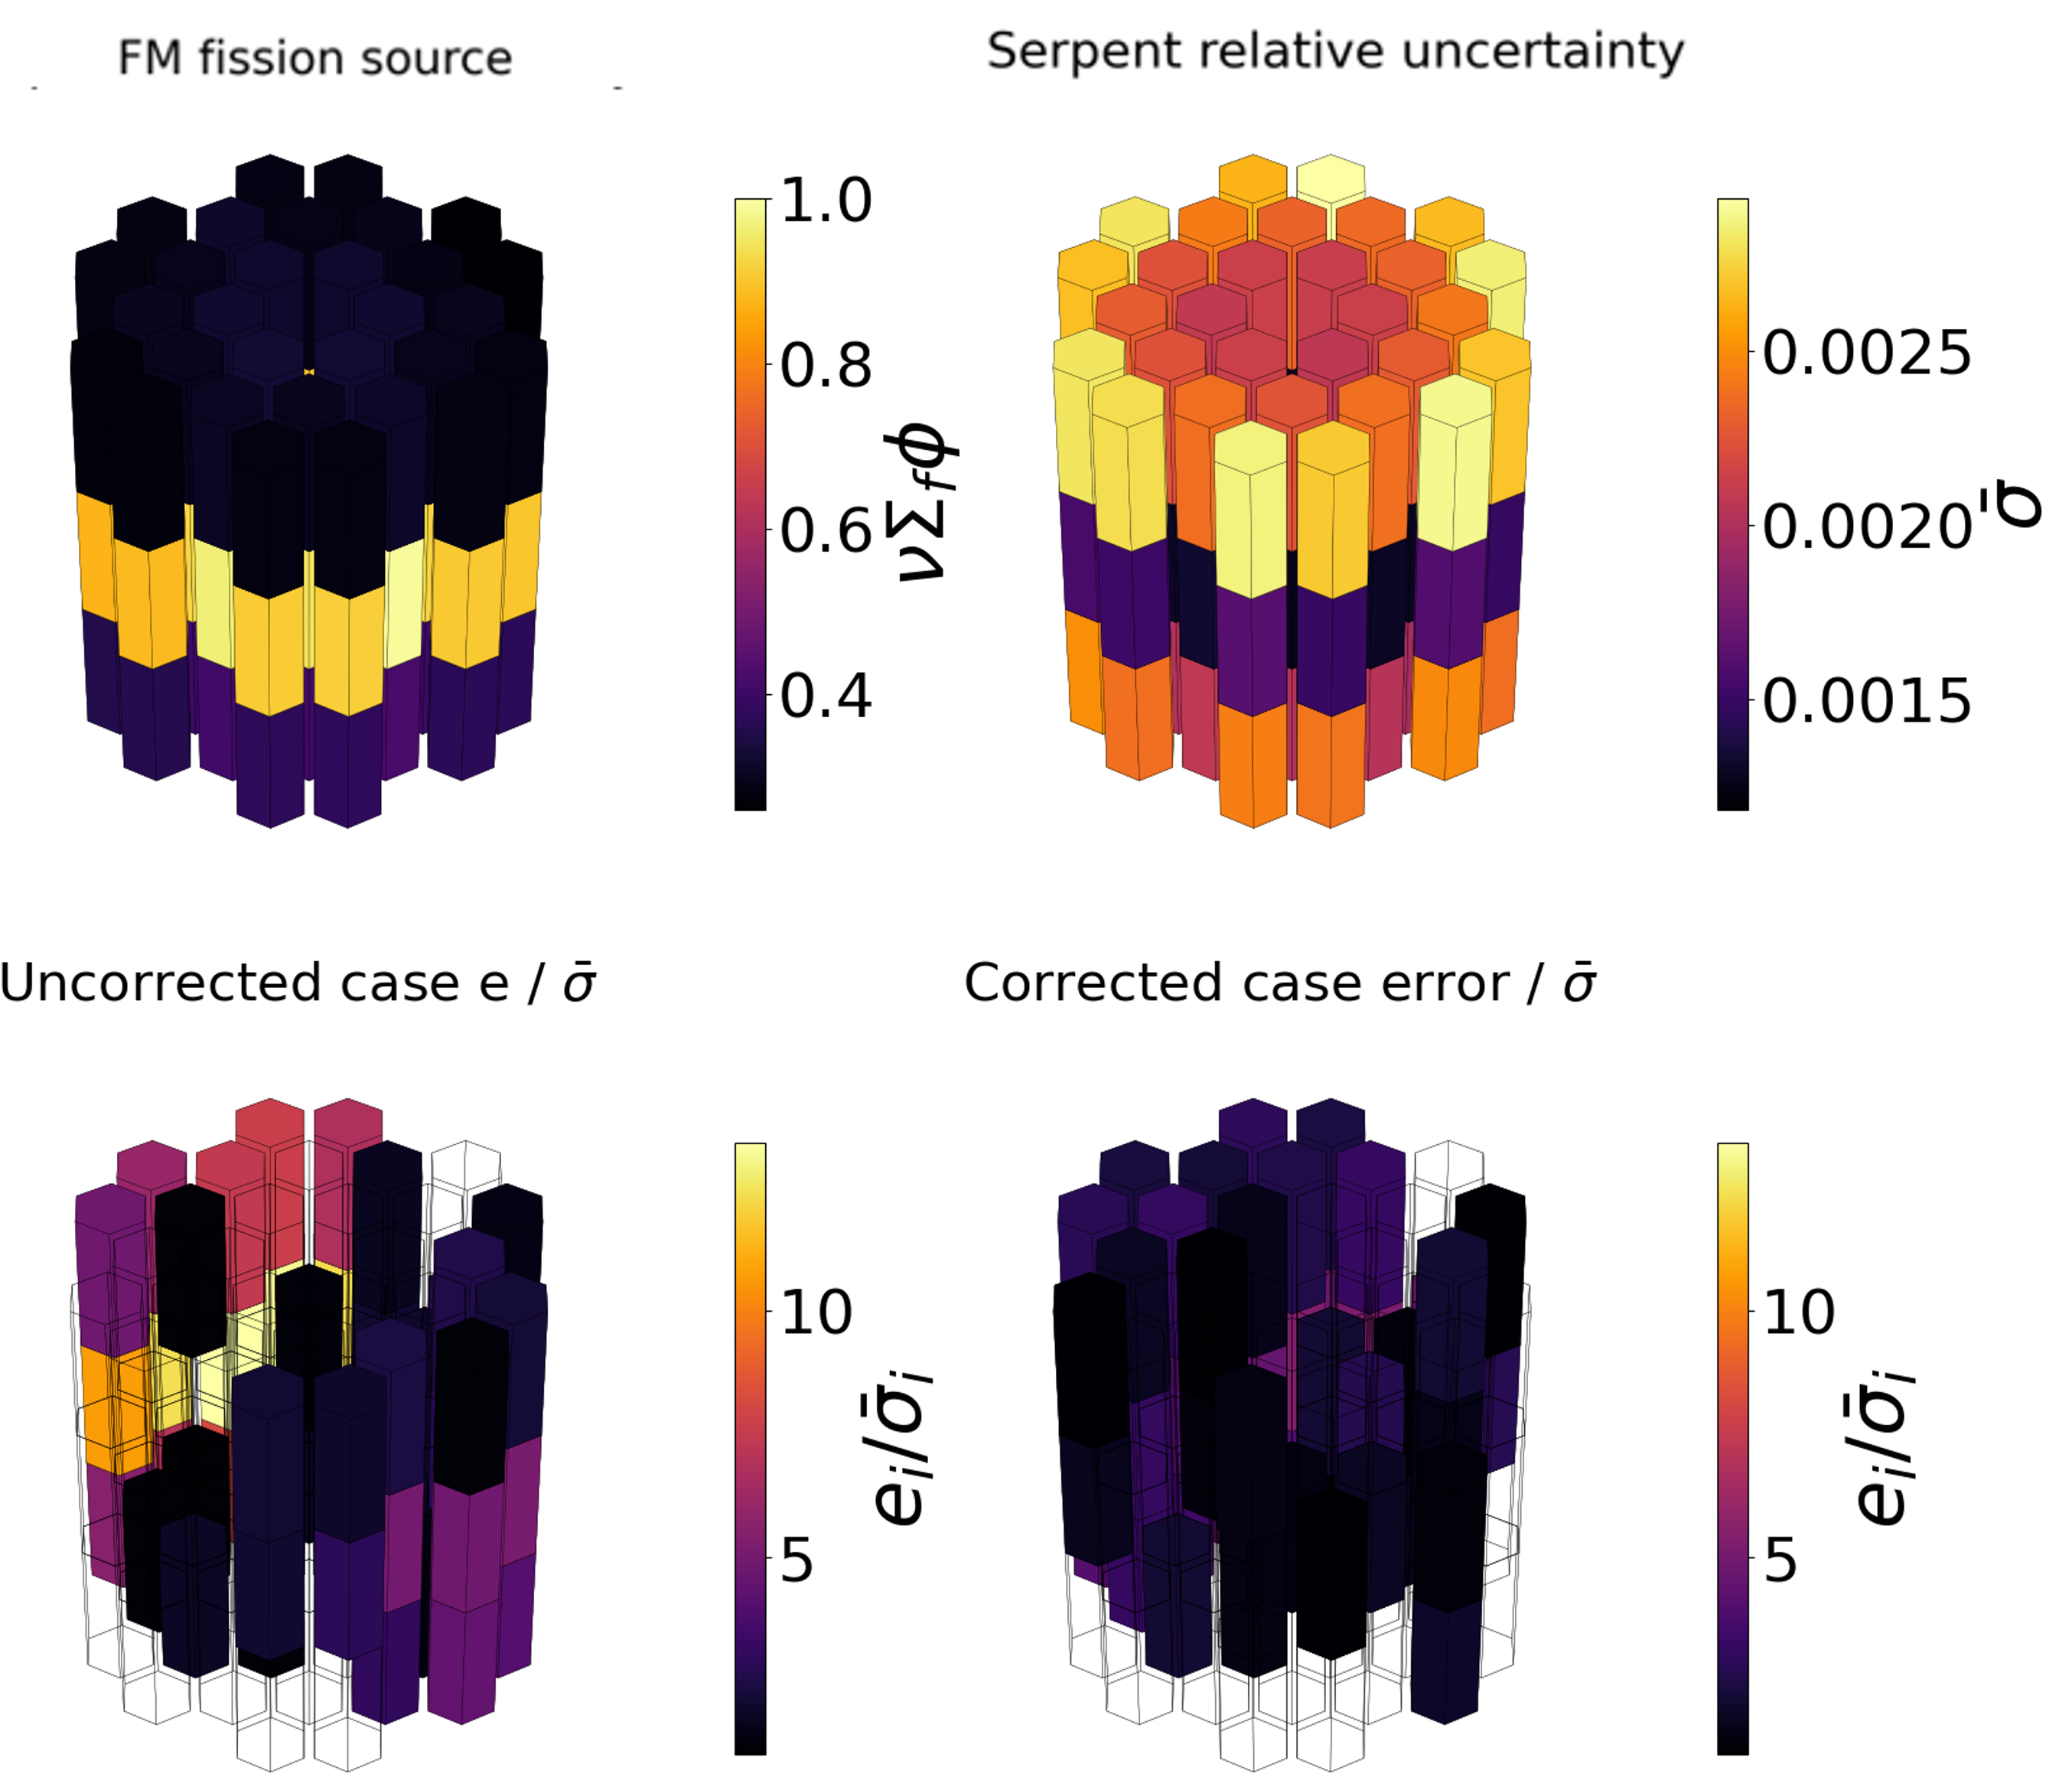
\includegraphics[scale=0.6]{images/Tf_linear_case_6.png}  % Modifica scale o usa width se serve
\caption{Case 6 of \cref{tab:testing_cases_5_6_7}. The corrected-case refers to the one using \cref{eq:correction_ratio_2} }
\label{fig:Tf_linear_case_6}
\end{figure}

\begin{figure}[h!]
\FloatBarrier
\centering
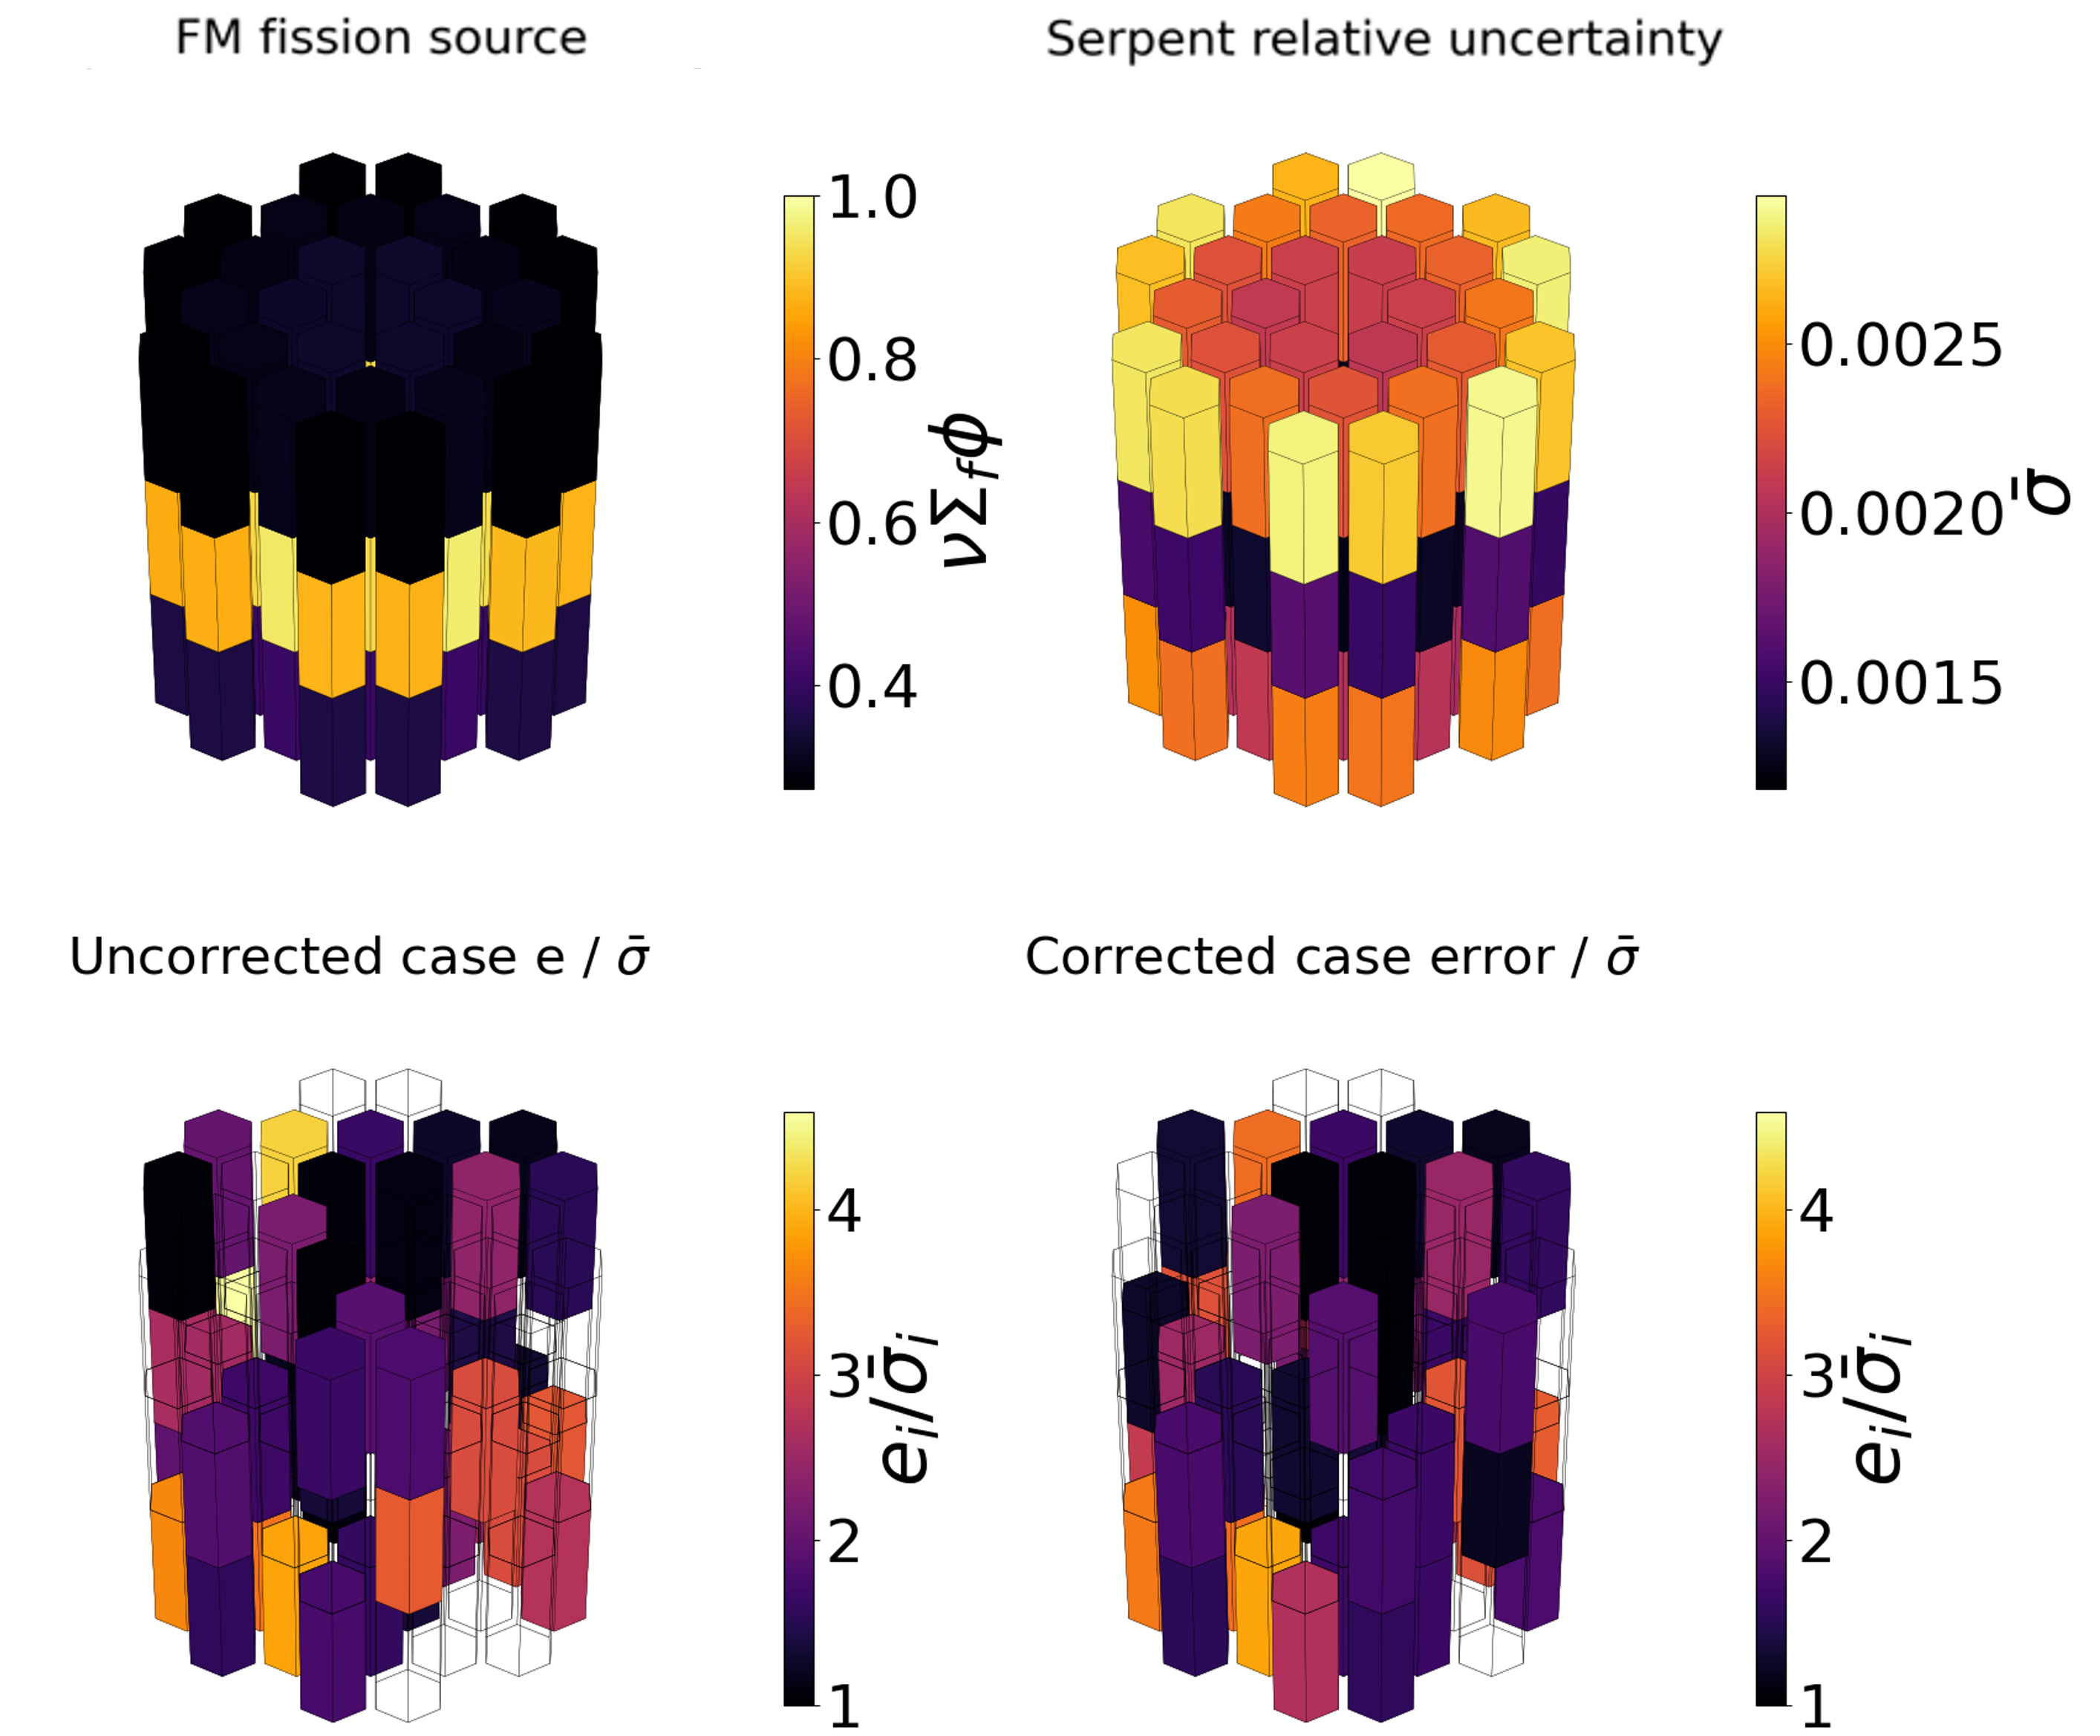
\includegraphics[scale=0.6]{images/Tf_power_like_case_7.png}  % Modifica scale o usa width se serve
\caption{Case 7 of \cref{tab:cases_testing_cases_for_gradient_T}. The corrected-case refers to the one using \cref{eq:correction_ratio_2} }
\label{fig:Tf_power_like_case_7}
\end{figure}


\subsection{Criticality search algorithm using the FM method}
 Relying on the good accuracy and the computational velocity of the FM method, a criticality search algorithm based on the FM method is defined as described in \cref{subsec:criticality_search_method}, as proposed also in \cite{Topham2020}. 

The power is given as an input to \cref{eq:correction_power_temperature}, where the parameters used to determine the formulation are the same of the case study 7, thus, based on realistic values. 
As can be observed in \Cref{fig:critical_CD_angle_VS_power}, the relation between the critical CDs angle and the power is linear. One could expect to have a less linear behaviour of curve, however it has to be stressed the fact that the thermal feedback effect is much less stronger compared to the CD worth.  

\begin{figure}[h!]
\FloatBarrier
\centering
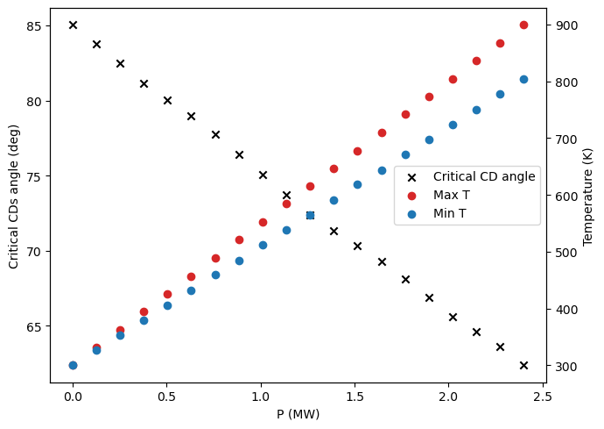
\includegraphics[scale=0.6]{images/critical_CD_angle_VS_power.png}  % Modifica scale o usa width se serve
\caption{Critical CDs angle for each of the twenty power values considered between 0 MW to 2.4 MW (black crosses). Respectively, the blue and red dots represent the minimum and maximum temperature value of the system at the corresponding power.  }
\label{fig:critical_CD_angle_VS_power}
\end{figure}

To verify if the critical CD angle calculated by the algorithm based on the FM is reliable, four additional test cases are considered, at the corresponding power levels: 0 MW, 0.8 MW, 1.6 MW, 2.4 MW, with the CDs rotated by their corresponding critical angle. In \cref{tab:testing_cases_8_9_10_11}, the results are reported. 

\begin{table}[h!]
\FloatBarrier
\caption{Testing cases at power levels: 0 MW, 0.8 MW, 1.6 MW, 2.4 MW.}
\centering
\begin{tabular}{llcccc}
\cline{3-6}
&                                                  & Case 8 & Case 9 & Case 10 & Case 11 \\ \hline
$\sigma_{k_{eff}}$ & \multicolumn{1}{l|}{CR}         &    16    &    19    & 15  & 17    \\ \hline
$\Delta k_{eff}$ (pcm)   
& \multicolumn{1}{l|}{$r_{ij}$ def.2}      &    23    &    38    & 19  & -20  \\ \hline
max($|e|$) (\%)     
& \multicolumn{1}{l|}{$r_{ij}$ def.2}    &    0.8   &   1.2     &     1.4   & 2.2 \\ \hline
RMSE (\%)         
& \multicolumn{1}{l|}{$r_{ij}$ def.2}    &      0.4  &   0.5   &   0.6     & 0.8 \\ \hline
\end{tabular}
\label{tab:testing_cases_8_9_10_11}
\end{table}


\section{Conclusions and Future Perspectives}

The presented results confirm that the Fission Matrix (FM) method, combined with appropriate correction ratios, provides a reliable estimation of reactivity parameters under a variety of thermal and geometrical conditions.

For this study a linear interpolation was adopted and  the database was selected by increasing the number of data till the error of the eigenvalue is sufficiently low, compared to the statistical uncertainty of the testing cases. The final database has 136 FMs, and each calculation required on average, 60 h/CPU. These calculations were performed on a PC equipped with an Intel® Xeon® Gold 6130 CPU @ 2.1 GHz, utilizing 30 cores., thus in total 272 h is the total computational time needed to obtain the database. However, the correction ratio defined to account for temperature difference between the active region and the reflector, leaded to 17 additional cases, increasing the computational burden to 306 h. 

In the first set of test cases with imposed temperature gradients between the core and reflector (\cref{tab:cases_testing_cases_for_gradient_T2}), significant deviations in $k_{eff}$ were observed when no correction was applied. In particular, $\Delta k_{eff}$ values exceeded 400 pcm in some configurations and the relative error of the fission source reaches higher value in the cells that directly face the reflector. The application of the correction ratio notably reduced such discrepancies, with RMSE values generally below 1\% and corrected $\Delta k_{eff}$ values falling within the uncertainty margins of the reference Serpent2 calculations.

In the extended test cases involving more complex and non-uniform temperature distributions (Cases 5--7, \cref{tab:testing_cases_5_6_7}), the method maintained a good levels of accuracy even for case with non-realistic high temperature gradient inside the system (Case 5,6). The results suggest that the proposed correction approach is applicable even when the temperature varies spatially inside the core. Case 7, in particular, based on a temperature distribution proportional to the fission source, yielded low errors across all evaluated metrics, indicating that the method remains effective under more realistic operating conditions.

The criticality search algorithm based on the FM approach was also tested across different power levels (Cases 8-11, \cref{tab:testing_cases_8_9_10_11}). The computed control drum angles produced reactivity results close to the target critical condition, with RMSE values under 1\% and maximum errors below 2.2\%. These outcomes suggest that the method can be used to support the estimation of critical configurations under varying thermal conditions with limited deviation from the reference Serpent2 results. 

In the future, the proposed method could be extended to transient analyses by computing the static reactivity at each time step of the point kinetics equations using the Fission Matrix approach, as suggested in \cite{Dalinger2024}. This would enable the evaluation of reactivity changes at each time step based on a 3D transport-informed model. Furthermore, to account for different transient scenarios, the method could be refined to consider the rotation of only a subset of CDs, rather than all of them simultaneously (\cite{Mascolino2022}). For longer time-scale transients, the effects of fuel burnup and xenon concentration will also be considered (\cite{Roskoff2018},\cite{Pungerčič}).




\bibliographystyle{elsarticle-harv} 
\bibliography{bibliography}

\end{document}


